\chapter{Related Work}
\label{chap:related_work}

This chapter reviews literature and existing work which is of relevance to this study. It is structured in 7 main sections:

\begin{enumerate}
    \item Review of digital and net art conservation theory
    \item Review of archival standards and systems
    \item Review of blockchain, smart contracts and NFTs
    \item Overview of the architecture of Teia and HEN OBJKTs
    \item Survey of representative artworks
    \item Tentative taxonomy of crypto art
\end{enumerate}

\vspace{0.5cm}

The review follows a narrative approach, with the goal of understanding the contextual background in which this work is situated. However it should be noted that there was a delimitation in the selection of materials reviewed, as only those which were made available as open access were included. In addition to academic papers, a number of books were reviewed, in the areas of blockchain art, netart, digital art conservation and information systems. A number of web resources in the area of art conservation were also consulted. 

Due to the novel area of networked crypto art, there is not a lot of existing academic literature published in this specific topic. For this reason, the research for this work relied primarily on the existing work of conservation of the Web, the extensive literature on digital art conservation in general, particularly that which focused on code-based art and netart, and also on a review of actual code-based crypto artworks.

\section{Digital and Net Art Conservation}

Due to the lack of existing literature on the conservation of networked crypto art, a reasonably good starting point is the study of digital art, and where possible, focusing on net art.

Net art is an art movement which started in the early 1990s and gained prominence in the middle of the decade, fuelled by the rise in popularity of the World Wide Web \cite{schreiberNetArtShedding2001}. It uses the Internet as a medium, and is usually highly interactive often invoking the participation of the viewer \cite{kholeifInternet_ArtBirthWeb2023}. Although there is no clear consensus on a definition of net art, this study will adopt the definition proposed by Rhizome on their Net Art Anthology: "art that acts on the network, or is acted on by it" \cite{WhatNetArt2017}.
This emphasis on the interaction between the art and the network was famously captured by MTAA in 1997, see \autoref{fig:simplenetartdiag}.

\begin{figure}[h]
    \centering
    \captionsetup{justification=centering}
    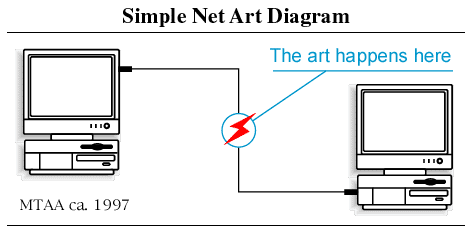
\includegraphics[width=0.75\linewidth]{netartdiagram.png}
    \caption[Simple Net Art Diagram]{Simple Net Art Diagram. Source: MTAA \cite{NETARTANTHOLOGY2016a}}
    \label{fig:simplenetartdiag}
\end{figure}

Net art shares many similarities with networked crypto art. In fact, if we try to set them apart, the main difference between a net net artart artwork and a networked crypto art artwork is that the later is registered on a blockchain, and as per our delimitation of scope, operates exclusively in the digital realm. Thus crypto art can be said to lay at the intersection of net art and crypto art. This allows us to draw the first part of our conceptual framework.


\begin{figure}[h]
    \centering
    \captionsetup{justification=centering}
    \includesvg[width=0.75\textwidth]{netart-crypto-art}
    \caption[Networked crypto art at the intersection of net art and crypto art]{Networked crypto art is at the intersection of net art and crypto art}
    \label{fig:netart-crypto-art}
\end{figure}

Net art belongs to a wider category of digital art, specifically born-digital art, which designates artworks created in a digital format from the outset, and which depends on the technology to operate \cite{innocentiKeepingBitsAlive2013}.

\subsection{Conservation}

As defined in \autoref{sec:definitions} (\nameref{sec:definitions} , page \pageref{sec:definitions}), conservation consists of a number of activities taken toward achieving the long-term preservation of cultural heritage. There is a wide range of such activities, but after a systematic review of digital art conservation literature, the following emerged as the most common:

\begin{itemize}
    \item Aquisition
    \item Archival Storage
    \item Access
    \item Emulation
    \item Migration
    \item Restoration
    \item Reconstruction
    \item Reinterpretation
    \item Documentation
\end{itemize}

The following sections will examine these activities in more detail.

\subsection{Acquisition}

Acquisition is the process that a cultural heritage institution takes to obtain an artifact for conservation. It is normally divided into 3 phases \cite{ahtilaAcquiringMediaArt1998}:

\begin{enumerate}
    \item \textbf{Pre-aquisition}: a pre-assessment of the artifact, to find its condition and whether it can be exhibited sustainably. This assessment includes an estimation of the overall costs, which include acquisition, exhibition, and continuing costs. If the assessment is positive, then the terms for the negotiation of the acquisition contract are drafted.
    \item  \textbf{Acquisition}: the process of acquisition involves negotiation with the vendor or donor, verification that all agreed components were delivered, including preservation materials, and exchange contracts;
    \item  \textbf{Post-acquisition}: work is catalogued and documented, and a long term conservation plan is made, potentially informed by follow-up interviews with the artist.
\end{enumerate}

In a digital context, acquisition is also commonly called \emph{injest}, see \autoref{sub:oais}.

\subsection{Archival Storage}

Cultural heritage institutions involved in conservation of digital art need to develop a robust archival storage strategy. Depending on the size of the institution they may choose to invest in on-site storage, normally in server rooms designed for that purpose, or outsource it to specialised storage or cloud vendors, and in many cases for the purposes of redundancy, both.

In this area the National Digital Stewardship Alliance (NDSA) published authoritative guidelines for industry best practices, see \autoref{tab:ndsa-levels-of-digital-preservation}

These guidelines include the practice of \emph{file fixity}, which consists of the use of checksums or file hashing, as discussed in \autoref{sub:blockchain}, to ensure a file is ``fixed'' or unchanged. It also encourages a well known practice in the archival community known as \emph{Lots of Copies Keep Stuff Safe} (LOCKSS).

Institutions are also adopting storage information systems which comply with the \gls{oais} standard. This standard is of special interest to this work, so it will be examined in more detail in \autoref{sub:oais}.

\begin{table}[h!]
\centering
\captionsetup{type=table} % This makes the caption be treated as a table caption
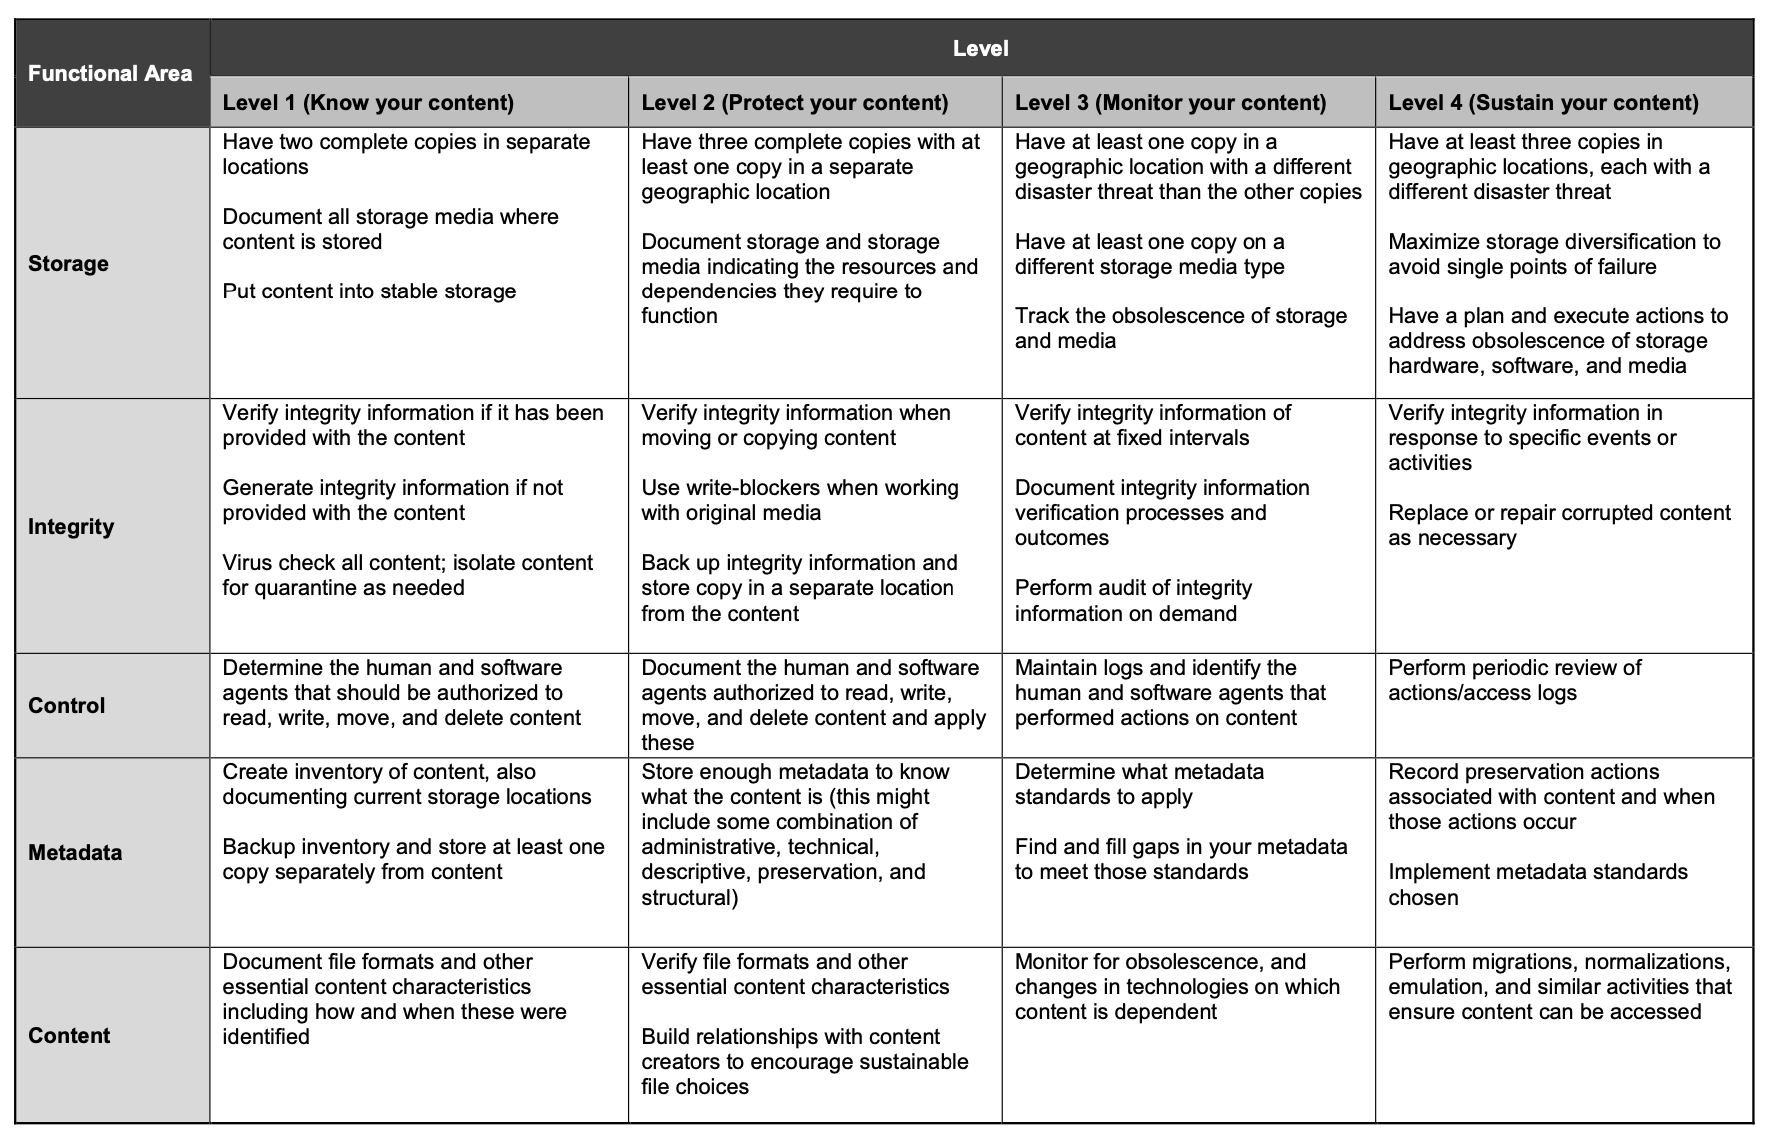
\includegraphics[width=\textwidth]{table-ndsa-matrix.png} % Adjust the width as needed
\caption[NDSA Levels of Digital Preservation Matrix V2.0]{NDSA Levels of Digital Preservation Matrix V2.0. Source: https://osf.io/qd54c}
\label{tab:ndsa-levels-of-digital-preservation}
\end{table}


\subsection{Access}

The archive should provide a user interface, allowing users to browse and search its contents, and in applicable to request copies of materials. In some cases some degree of access control may need to be put in place, in which case the system should provide such a feature. \cite{nationallibraryofaustraliaGuidelinesPreservationDigital2003}

\subsection{Emulation}

Emulation is the recreation of a particular system, either hardware or software, as software which runs in a virtualised environment within another system \cite{rothenbergUsingEmulationPreserve2000}. It is one of the most common methods of preserving digital systems which became obsolete over time.

It is widely used in a variety of contexts, from reviving old video games, such as arcade\footnotemark[1], ZX Spectrum\footnotemark[2], and many other obsolete systems\footnotemark[3], as well as more recent web publishing proprietary systems like Adobe Flash\footnotemark[4] and even obsolete calculators \cite{scottjasonCalculatedMoveCalculators2023}.

\footnotetext[1]{\url{https://www.mamedev.org/}}
\footnotetext[2]{\url{https://archive.org/details/softwarelibrary_zx_spectrum}}
\footnotetext[3]{\url{https://archive.org/details/software}}
\footnotetext[4]{\url{https://ruffle.rs/}}

OldWeb.Today, which combines web-based \gls{emulation} of obsolete browsers, like NCSA Mosaic and Netscape Navigator, with Archive.org's Wayback Machine web snapshots, enables users to experience navigating the web as it was all the way back into the 1990s, see \autoref{fig:oldweb}.

\begin{figure}[h]
    \centering
    \captionsetup{justification=centering}
    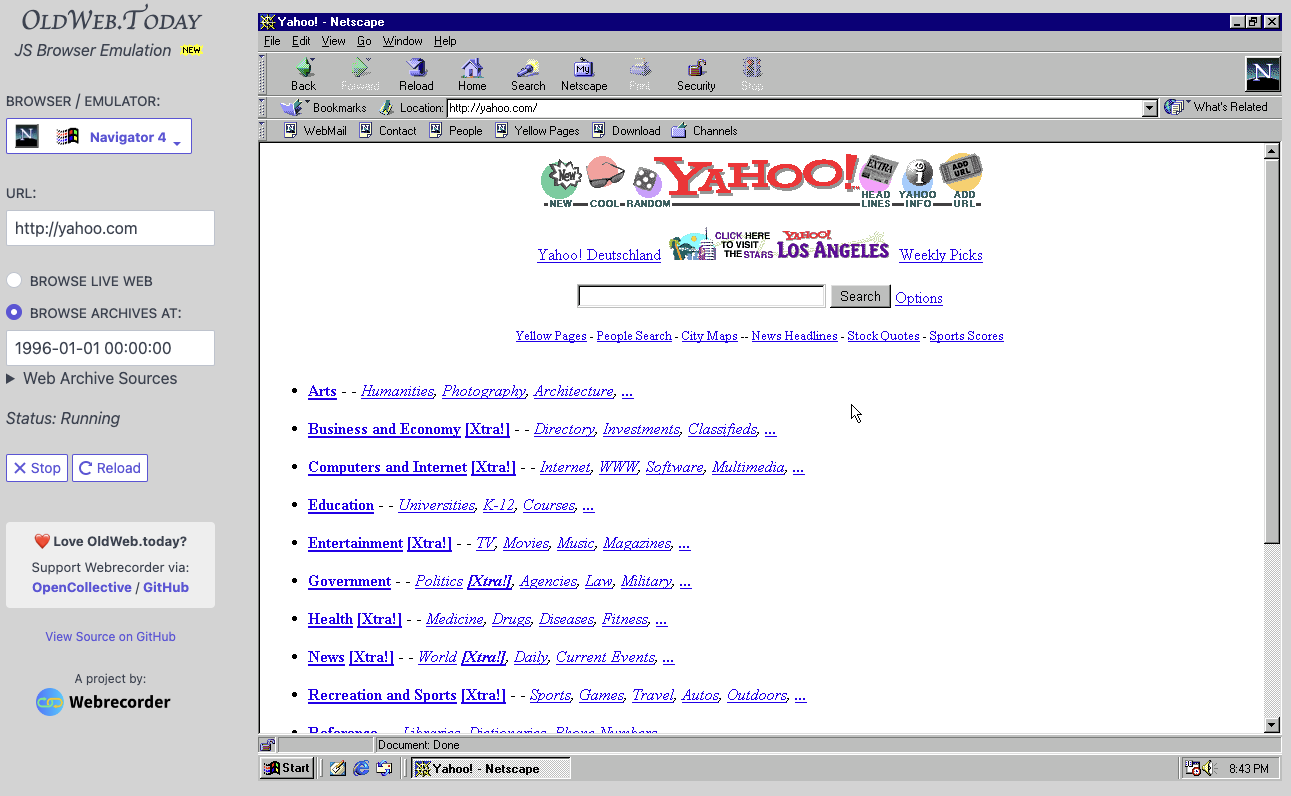
\includegraphics[width=\linewidth]{oldweb.png}
    \caption[OldWeb.Today Browser Emulator]{OldWeb.Today Browser Emulator. Source: https://oldweb.today/ }
    \label{fig:oldweb}
\end{figure}

One challenge of emulators is that, as any other software system, they may have to be readapted to run on more modern hardware. This means that the work of creating and updating emulator software is likely to be an ongoing effort for the foreseeable future.

\subsection{Migration}

Migration of a digital artwork involves moving it from its original technological environment, to a more modern one. However it is often the case that this will result in some degradation of the artwork, due to incompatibilities between the two environments. \cite{huberNewMediaOld2013}

As an empirical example of this, we can use the ACID test v2, which was test web page setup in 2005 by the Web Standards Project to test web browser compatibility with the standards for displaying HTML markup, PNG images, CSS 2.1styling, and data URIs \cite{Acid22024}.

If we access the test page\footnotemark[5] with a modern browser, such as Google Chrome Version 127 on a Mac OS 13.6 operating system, and compare it with the reference image\footnotemark[6], we can see clearly that backwards compatibility with web standards that were in place less than 20 years ago is already decaying.

\footnotetext[5]{\url{http://acid2.acidtests.org/\#top}}
\footnotetext[6]{\url{http://acid2.acidtests.org/reference.html}}

\begin{figure}[h]
  \centering
  \begingroup
  \setlength{\fboxsep}{0pt} % No padding between box and content
  \setlength{\fboxrule}{1pt} % Thickness of the border
  \begin{subfigure}[b]{0.45\textwidth}
    \centering
    \fcolorbox{gray}{white}{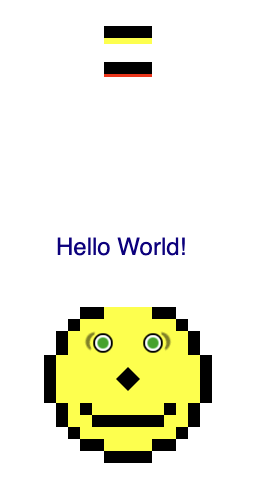
\includegraphics[width=\textwidth]{acid2-test.png}}
    \caption{ACID test v2 in 2024}
    \label{fig:acid1}
  \end{subfigure}
  \hfill
  \begin{subfigure}[b]{0.45\textwidth}
    \centering
    \fcolorbox{gray}{white}{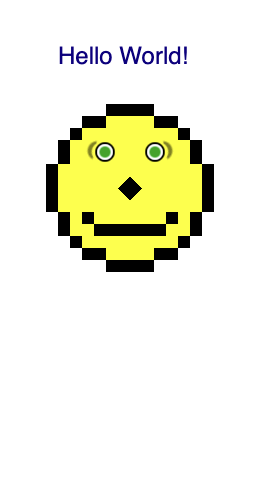
\includegraphics[width=\textwidth]{acid2-reference.png}}
    \caption{ACID test v2 reference image}
    \label{fig:acid2}
  \end{subfigure}
  \endgroup
  \caption{ACID v2 test with modern browser}
  \label{fig:acid2-test}
\end{figure}


This is a reminder that following web standards today is no guarantee of the fidelity of renderings in the future. 

\subsection{Restoration}

Restoration is an umbrella term used for a set of conservation practices "undertaken to restore an object to known preceding states" \cite{dekkerCollectingConservingNet2018}. In general these are meant to be as non-invasive as possible in order to maintain the artworks' authenticity. 

\subsection{Reconstruction}

Reconstruction goes a step further than restoration, as it involves rebuilding parts of an artwork, usually based on extensive documentation provided by the artist, so as to maintain their original intent, although it can be argued that any reconstruction is always susceptible to some degree or reinterpretation \cite{huberNewMediaOld2013}.


\subsection{Reinterpretation}

Reinterpretation represents the most radical intervention in the integrity of an artwork, as it may need to be adapted to a new environment, with new parameters. It may sometimes present itself as the last resort to preserve the artwork and, just like reconstruction, ideally it should be done in consultation with the artists as to maintain its original intention \cite{serexheDigitalArtConservation2013}.


\subsection{Documentation}

Documentation is arguably the most important conservation practice in digital art preservation, being mentioned in the vast majority of articles and books.

Depocas noted that ``sometimes this documentation is the only evidence left of an artwork's existence'' \citeyear[p.145]{depocasDocumentingConservingTechnological2013}.

Several efforts have been initiated by digital art conservation community in an effort to standardise documentation practices.

\subsubsection{Variable Media Network}

The Variable Media Network is a project that provides a set of guidelines and taxonomies, and a questionnaire which can help guide conservators in documenting digital artworks \cite{depocasPermanenceChangeVariable2003}. For example, artworks can be classified as: contained, installed, performed, interactive, reproduced, interchangeable, encoded (our definition of code-based), and networked. Their questionnaire allows the recording of elements such as: stakeholders (persons, institutions, studios), artworks (title, year, description), components (material, environment, interaction), package (contained, installed, performed, interactive), questions (about storage, emulation, migration, reinterpretation), and allows the linking of these elements. For example a stakeholder, like an artist, can be linked to several artworks \cite{VariableMediaNetwork}.

The project also implemented a questionnaire\footnotemark[7] as an interactive web-based application, as illustrated in \autoref{fig:vmnq}.

\footnotetext[7]{https://variablemediaquestionnaire.net/}

\begin{figure}[h]
    \centering
    \captionsetup{justification=centering}
    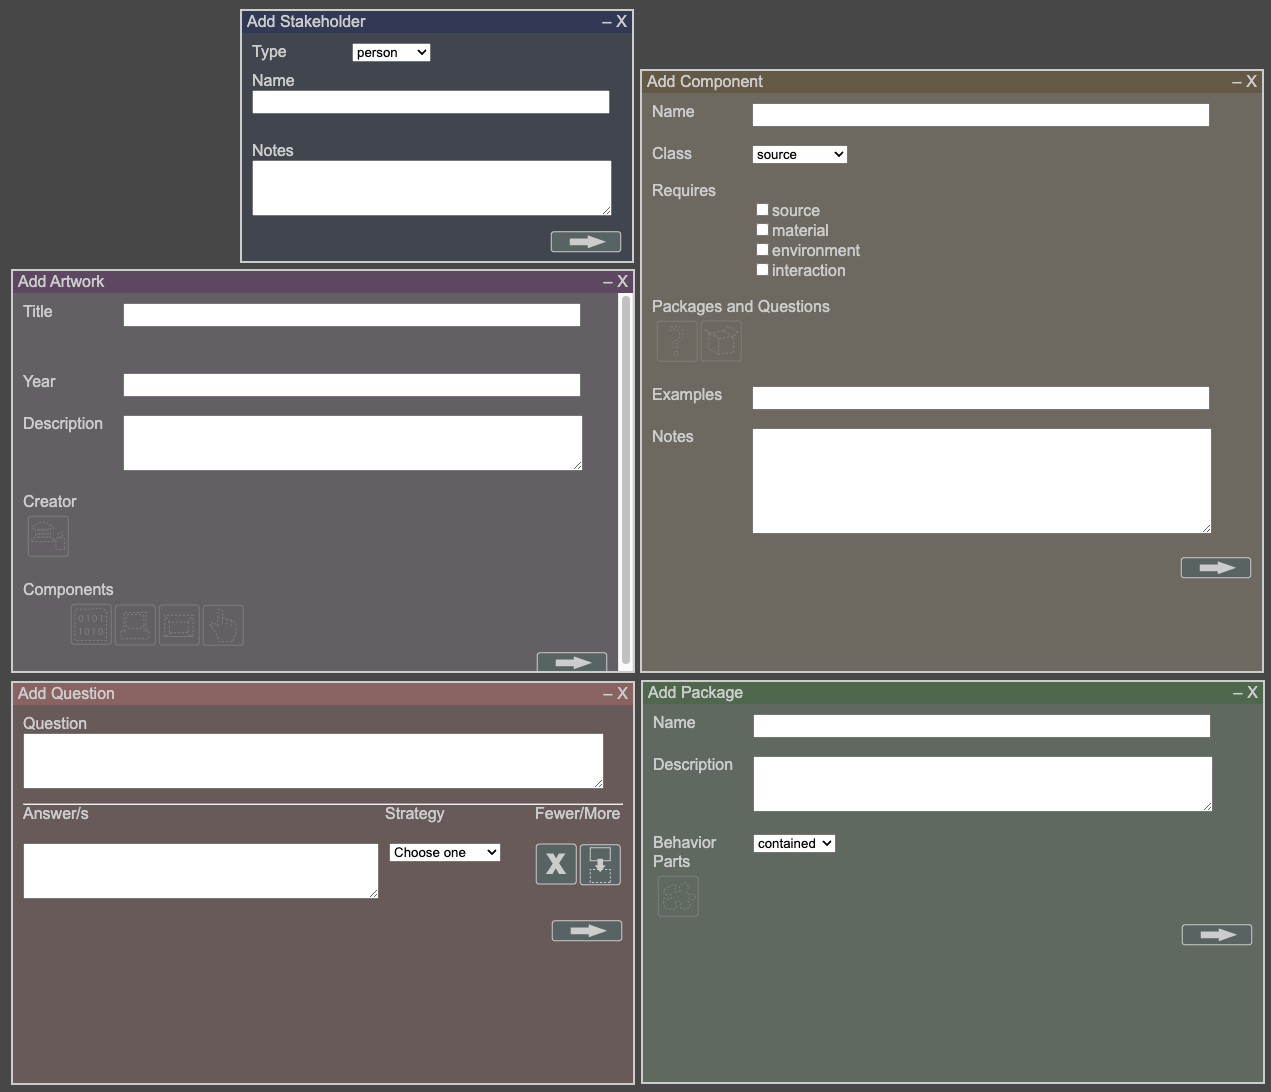
\includegraphics[width=\linewidth]{variablemedianet-questionnaire.png}
    \captionsetup{justification=centering}
    \caption[Variable Media Network Questionnaire]{Variable Media Network Questionnaire. \\ Source: https://variablemediaquestionnaire.net/}
    \label{fig:vmnq}
\end{figure}

\subsubsection{DOCAM Documentation Model}

The Research Alliance Documentation and Conservation of Media Arts Heritage \cite{DOCAM} produced cataloguing and conservation guides, as well as a set of documentation models for the conservation of media art. This model ``offers a structural framework within which all the information pertaining to a work can be assembled, organized, and made accessible'' \cite[p.151]{depocasDocumentingConservingTechnological2013}.

Their model structures the documentation across 4 main lifecycles of the artwork: creation, dissemination, research and custody. See \autoref{fig:docam-model}.

\begin{itemize}
    \item \textbf{Creation}: definition of the concept, presentation method, and required elements its presentation;
    \item \textbf{Dissemination}: presentation and publicity strategies, including installation, presentation, deinstallation and criticism;
    \item \textbf{Research}: activities surrounding the study or critical analysis of a work;
    \item \textbf{Custody}:  various facets of custodial responsibility, such as storage, cataloguing, conservation and preservation;
\end{itemize}


\begin{figure}[h]
    \centering
    \captionsetup{justification=centering}
    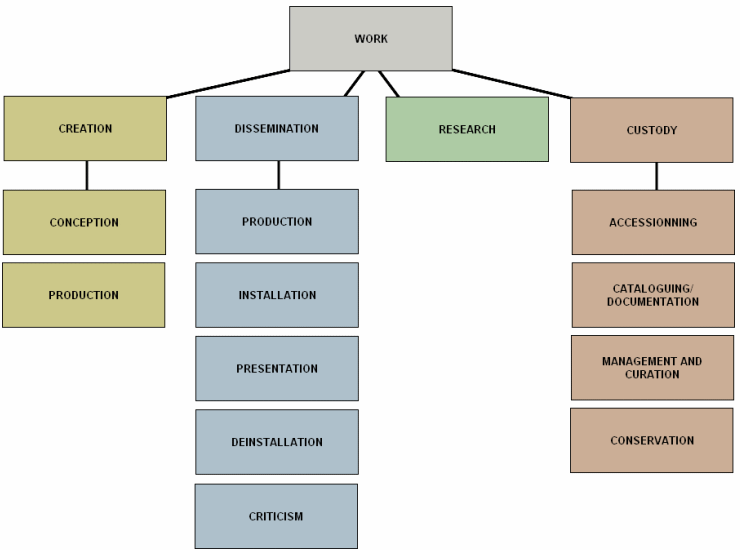
\includegraphics[width=\linewidth]{docam-struct.png}
    \captionsetup{justification=centering}
    \caption[DOCAM Documentation Model - Lifecycle Events]{Lifecycle events of a work as per the DOCAM Documentation Model. \\ Source: https://www.docam.ca/en/documentation-model.html}
    \label{fig:docam-model}
\end{figure}


\section{Archival Standards and Systems}

Digital preservation is not a problem specific to digital art, and several efforts have been made to create standards for the long-term archival of digital assets. The following sections discuss some of the most significant ones.

\subsection{Open Archival Information System (OAIS)}
\label{sub:oais}

The Open Archival Information System (\gls{oais}), an ISO standard, is the standard reference model for the long term archiving of digital data, and is one of the most quoted archival standards in digital art preservation. Its model describes best practices across all stages of a digital asset's life cycle: ingest, archival storage, data management, and access \cite{ccsdsReferenceModelOpen2012}. These stages were taken into account when developing the artifact for this project.

The model makes reference to 3 types of information packages:

\begin{itemize}
    \item \textbf{Submission Information Package (SIP)}: which is the information sent from the producer to the archive 
    \item \textbf{Archival Information Package (AIP)}: which is the information stored by the archive
    \item \textbf{Dissemination Information Package (DIP)}: which is the information sent to a user when requested
\end{itemize}

It also makes recommendations with regards to the metadata that should be attached to each digital asset:

\begin{itemize}
    \item reference (identification) information
    \item provenance (including preservation history)
    \item context
    \item fixity (file checksums)
    \item representation (formatting, file structure)
\end{itemize}


\begin{figure}[h]
    \centering
    \captionsetup{justification=centering}
    \includesvg[width=\textwidth]{OAIS-high-level-data-flow}
    \caption[OAIS High Level Data Flow]{OAIS High Level Data Flow. \\ Adapted from: https://public.ccsds.org/Pubs/650x0m2.pdf}
    \label{fig:oais-high-level-data}
\end{figure}

This model constitutes the gold standard for digital archives, and is quite applicable to an archive of crypto art such as the one developed by this project. As mentioned above, at a very basic level \texttt{ARKIVO} already implements the high level data flows illustrated in \autoref{fig:oais-high-level-data}. However a great deal of work is still required to address aspects of the standard such as migration, interoperability and others.

\subsection{Archivematica}

Archivematica\footnotemark[8] is a web-based digital archive that follows the OAIS standard and integrates with many other data repository systems. It is open source, well designed and reasonably well maintained. However it was not suitable as a base software stack for this project because it relies heavily on web2 style authentication (username and password) and therefore it does not suit the web3 culture that our artifact needs to cater for.

\footnotetext[8]{https://www.archivematica.org/en/}

\subsection{Rhizome ArtBase}

The Rhizome ArtBase is an online archive of digital artworks. At the time of writing it hosts 2318 artworks, ranging from websites, moving images, net art, code-based artworks, and games.

Following are screenshots of the main landing page, and an artwork page.


\begin{figure}[H]
  \centering
  \captionsetup{justification=centering}
  \begin{subfigure}[b]{0.45\textwidth}
    \centering
    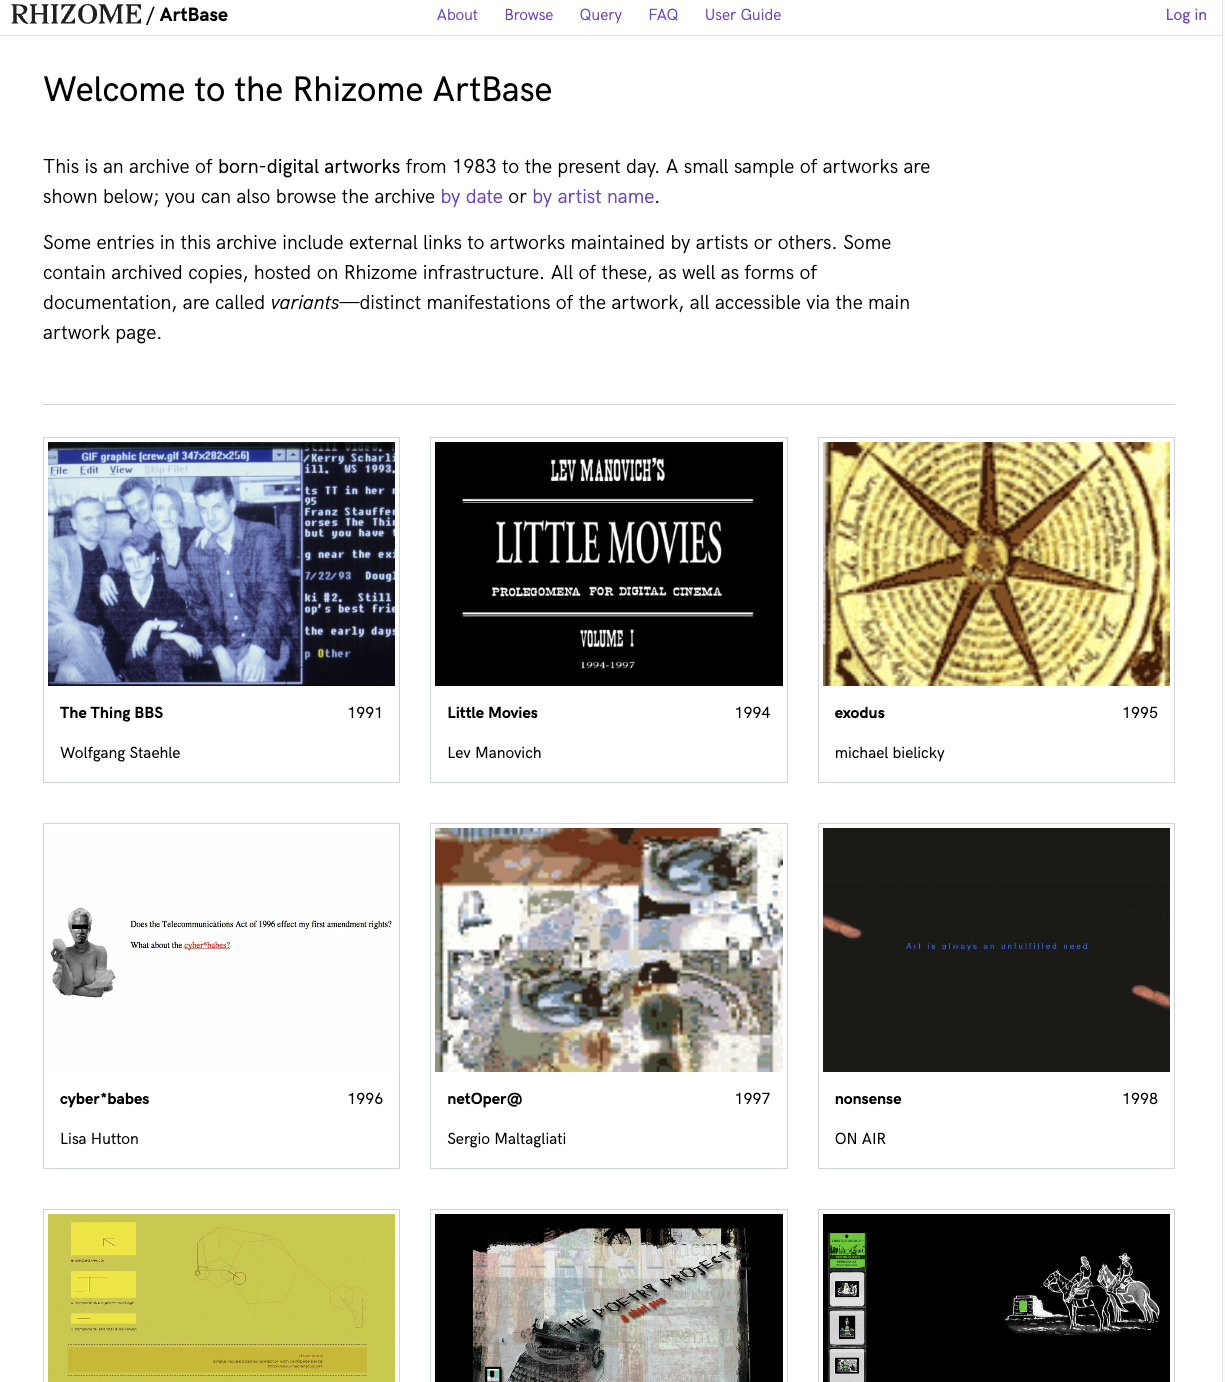
\includegraphics[width=\textwidth]{rhizome-artbase.png}
    \caption{Rhizome ArtBase}
    \label{fig:image1}
  \end{subfigure}
  \hfill
  \begin{subfigure}[b]{0.45\textwidth}
    \centering
    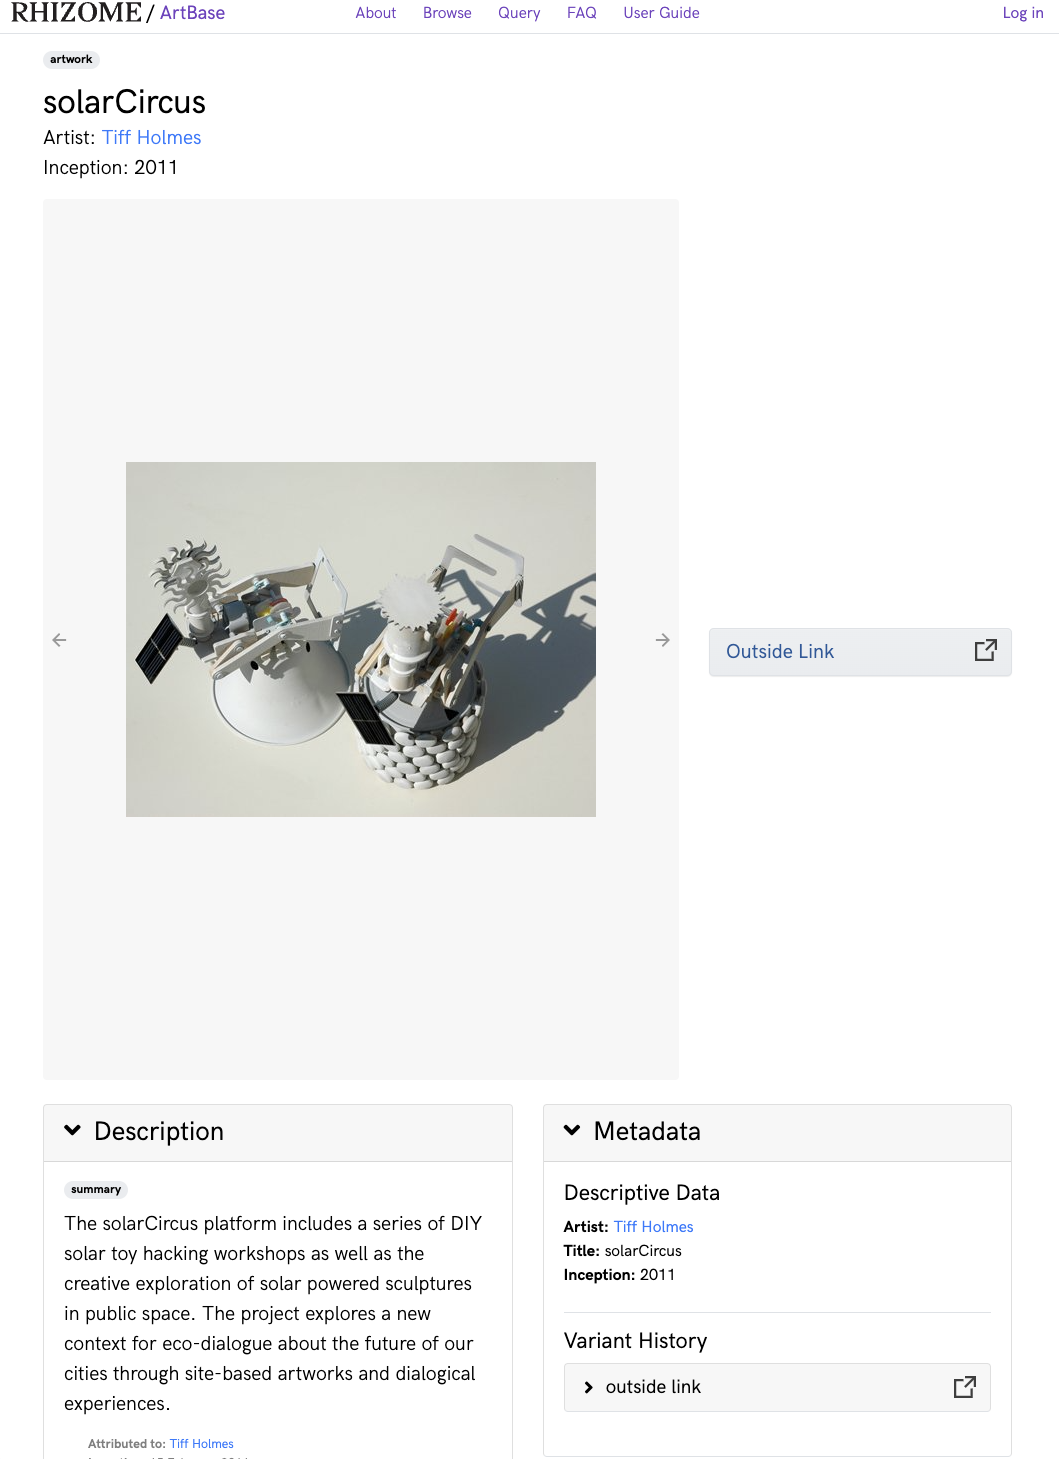
\includegraphics[width=\textwidth]{rhizome-artwork.png}
    \caption{solarCircus by Tiff Holmes}
    \label{fig:image2}
  \end{subfigure}
  \caption{Screenshots of Rhizome ArtBase. \\ Source: https://artbase.rhizome.org/}
  \label{fig:rhizome-screens}
\end{figure}

Each artwork page contains a basic description, and additional metadata about the artwork. It also contains linked objects (normally to the artist's own website), archival copies, or both.

It does not provide a traditional search function, but rather a more powerful query service based on the SPARQL query language, which in theory should allow for complex queries of its Linked Open Data (LOD) infrastructure. However at the time of writing this feature fails run, even the demo queries provided by the system.

Its minimalistic design, which places the artwork first, was a major inspiration for the artifact developed in this work. 

\subsection{Archive.org and Wayback Machine}

Although not specific to art, archive.org undoubtedly constitutes one of the most important archives of web history. It currently hosts 212 PetaBytes worth of web page snapshots, digitised books, videos, audio, images and software \cite{InternetArchivePetabox}.

Unfortunately, due to Teia's client-side and highly dynamic UI, Wayback Machine fails to capture any artworks rendered on Teia's main pages. According to the LOCKSS principle, this is unfortunate, as having another archival copy of the artworks would be advantageous. Although it's possible to manually request snapshots of the IPFS asset itself, bypassing Teia's UI, in practice it would make finding such an artwork very difficult, as most users would be looking for the snapshots of the Teia URLs.

\subsection{WebRecorder and WARC files}

The WebRecorder project develops a number of tools for the recording (archival), and replaying, of webpages, similarly to the snapshots taken by Wayback Machine. These tools range from browser extensions, to desktop applications, and even command line tools and software libraries.

Importantly, snapshots taken by the WebRecorder family of tools conform to the Web ARChive (WARC) file format, which has become a standard in the industry \cite{WARCFileFormat2024}.

Such a feature would be highly valuable for our artifact, however through experimentation it was found that, unlike their desktop tools, the software libraries currently lack the ability to fully capture a web page with all its assets. Instead they only capture a single HTTP request. Lacking this basic single-page crawling ability meant that integration of WARC snapshots will be postponed for future work.


\section{Blockchain Technology, Smart Contracts and NFTs}


\subsection{Blockchain}
\label{sub:blockchain}

The concept behind a blockchain is not new. It was first introduced by Stuart Haber and Scott Stornetta in 1991 in the Journal of Cryptology \cite{haberHowTimeStampDigital1991}. The problem they were trying to solve was: how can we trust historical records when digital media is so easy to manipulate, and how can we do so without having to trust a central authority? Their solution relied on one-way hashing functions.


\begin{figure}[h]
    \centering
    \captionsetup{justification=centering}
    \includesvg[width=0.5\textwidth]{hashing}
    \caption[One-way hashing examples]{Examples of one-way hashing (here SHA1 was used). The same input always produces the same hash. Different inputs produce different hashes, even if the difference is just one character, or even one bit.}
    \label{fig:hashing}
\end{figure}

Haber and Stornetta's solution involved combining the hash of a document into the data input for the next document hash, resulting in a recursive chain of hashes which had an important property: any change to any of the documents, no matter how small, would break the chain of hashes from that point onwards.
By weekly publishing the latest hash of the chain, which they did in the``Notices'' classified advertisements section of a the New York Times \cite{whitakerArtBlockchainPrimer2019}, they effectively created the first time-stamped proofs of the immutability of those digital documents, and arguably the world's first blockchain.

\begin{figure}[h]
    \centering
    \captionsetup{justification=centering}
    \includesvg[width=0.5\textwidth]{hash-chains}
    \caption[Illustration of a chain of hashes]{Illustration of a chain of hashes}
    \label{fig:hashing}
\end{figure}


\subsection{Bitcoin}

Satoshi Nakamoto \cite{nakamotoBitcoinPeertopeerElectronic2008a}  adopted this concept of an immutable data chain and added the required components to turn it into a global decentralised ledger, where financial transactions can be recorded. These components were:

\begin{enumerate}
    \item a peer-to-peer network of nodes running the same software, which validate all transactions added to the ledger 
    \item cryptographic signatures, so that transactions spending or transferring a particular asset are only accepted by the network when signed by the asset's owner
    \item the ordering of transactions into blocks, which are linked together by their hashes
    \item a lottery system that determines which node on the network is eligible to publish the next block
    \item a proof-of-work system with self-adjusting difficulty so that on average only one node is able to win the lottery every 10 minutes. Also the proof-of-work required for altering old blocks becomes exponentially larger with each block added, as an attacker would need to produce more proof-of-work than the rest of the honest nodes combined
    \item a fungible token, bitcoin, which is used to economically reward nodes who successfully publish blocks and is the native asset traded on the ledger
    \item in addition to block rewards, block producing nodes (miners) also receive fees paid by each transaction which was included in their block
\end{enumerate}

\vspace{0.5cm}

Although the blockchain contains a full history of all transactions ever made since its inception, Bitcoin stores the current state of the ledger, in other words, the index of who owns what, in a set of unspent transaction outputs (\indexacronym{utxo}). As the name suggests, this is the list of all transactions which have not yet been spent by their recipients.

With his invention, Bitcoin, Satoshi created the first decentralised cryptocurrency, which exhibits several key properties:

\begin{enumerate}
    \item \textbf{Decentralisation}: peer-to-peer network of nodes, operates without any central authority
    \item  \textbf{Censorship resistance}: transactions cannot be stopped of censored by any central authority
    \item  \textbf{Permissionless}: anyone with access to the Internet can download the software and participate on the network
    \item  \textbf{Immutability}: transactions added to the blockchain become immutable, as explained above
    \item  \textbf{Transparency}: all transactions on the ledger are public, and independently verifiable, removing the need for trust (trustless)
\end{enumerate}

\vspace{0.5cm}


\subsection{Ethereum}

As mentioned in the Introduction, Ethereum built on the concept of a blockchain, but unlike Bitcoin it does not use a UTXO approach. Instead, it uses an account-based model as a representation the state of the ledger. There are two types of accounts in Ethereum: Externally Owned Accounts (EOAs) which are controlled by a person's private key and are used to send and receive assets; and Contract Accounts which contain code that gets executed when it receives a transaction from an EOA. The code is executed by the Ethereum Virtual Machine (EVM) which makes changes to the persistent state storage, see \autoref{fig:smartcontract}.

\begin{figure}[h]
    \centering
    \captionsetup{justification=centering}
    \includesvg[width=0.75\textwidth]{smartcontract}
    \caption[Diagram of Smart Contract]{Diagram of Smart Contract}
    \label{fig:smartcontract}
\end{figure}

Just like in Bitcoin, transactions in Ethereum must pay a fee to the block producers, called gas fee. In the case of interactions with smart contracts, the gas is consumed during the execution of the code, with each instruction (opcode) costing a varying amount of gas corresponding to the computational complexity of that instruction. Any unused gas is returned back to the EOA. Gas is paid in Gwei, which is a denomination of Ether, Ethereum's native cryptocurrency.

Ethereum standards, like ERC-20, allow the creation of fungible tokens which can be traded across different wallets and \gls{decentralised application}s (\indexacronym{dapp}s) built on Ethereum \cite{ERC20TokenStandarda}, which led to the \gls{initial coin offering} (\indexacronym{ico}) hype of 2017 \cite{cuffeRoleErc20Token2018}.


\subsection{Non-Fungible Tokens}

The ERC-721 standard is used for the creation of unique and non-divisible NFTs, each with a unique identifier, such that they are not fungible as their ERC-20 counterparts.
Due to the limited storage available on the blockchain, the ERC-721 standard defined as part of its \texttt{ERC721Metadata} a \texttt{tokenURI} field which should point to an external location where the actual NFT metadata should be stored. In turn, this metadata should follow the ERC721 Metadata JSON Schema, and includes the name and description of the NFT, and another URI, this time to the actual NFT media asset \cite{ERC721NonFungibleToken}.

\begin{lstlisting}[language=, caption={ERC721 Metadata JSON Schema}]
{
    "title": "Asset Metadata",
    "type": "object",
    "properties": {
        "name": {
            "type": "string",
            "description": "Identifies the asset to which this NFT represents"
        },
        "description": {
            "type": "string",
            "description": "Describes the asset to which this NFT represents"
        },
        "image": {
            "type": "string",
            "description": "A URI pointing to a resource with mime type image/* representing the asset to which this NFT represents. Consider making any images at a width between 320 and 1080 pixels and aspect ratio between 1.91:1 and 4:5 inclusive."
        }
    }
}
\end{lstlisting}

Even though some early NFT marketplaces stored their NFT metadata and assets in private servers, leading to a loss of the assets when they shutdown \cite{gallenHistoryNFTMarketplaces2023}, nowadays most marketplaces store these in decentralised file storage networks like IPFS and ArWeave, which are more resilient  see \autoref{sec:offchain_storage} (\nameref{sec:offchain_storage}, \pageref{sec:offchain_storage}).


\begin{figure}[h]
    \centering
    \captionsetup{justification=centering}
    \includesvg[width=\textwidth]{nft-diagram}
    \caption[Components on an NFT on on Ethereum]{Components on an NFT on Ethereum}
    \label{fig:nftcomponents}
\end{figure}

\subsection{Off-Chain Storage}
\label{sec:offchain_storage}

As mentioned above, in order to avoid single-points of failure while storing NFT assets off-chain, most NFTs use decentralised file storage solutions to store their assets. Several projects offer such solutions, but lately two projects have gained relevance in this area: \gls{interplanetaryfilesystem} and ArWeave. 

\subsubsection{InterPlanetary File System}
\label{sec:ipfs}

IPFS is a suite of protocols for organising and transferring data over a \gls{peertopeer} network, using content addressing rather than location addressing, such as domain names or IP addresses.
Content addressing works by hashing the contents of the file, or smaller chunks (or blocks) when the file is big enough, see \autoref{fig:ipfs-cid-gen}. This hash is known in IPFS as a \gls{contentidentifier}. IPFS then uses these CIDs to organise the assets in a Merkle \gls{directed acyclic graph} allowing for efficient storage and retrieval. There are several reasons why files are split into smaller chunks, including faster parallel downloading from multiple nodes, and improving the changes of finding identical chunks between different files, which allows for chunk deduplication and hence savings in terms of storage space. \cite{juBlockchainTraceabilitySystem2022}

\begin{figure}[h]
    \centering
    \captionsetup{justification=centering}
    \includesvg[width=0.5\textwidth]{ipfs-cid-gen.svg}
    \caption[Generation Principle of CID in IPFS]{Generation Principle of CID in IPFS. Source: \cite[p.3]{juBlockchainTraceabilitySystem2022}}
    \label{fig:ipfs-cid-gen}
\end{figure}

CIDs are mapped onto the nodes (peerIDs) which host them, using a \gls{distributed hash table}. Through network gossiping the nodes can quickly find a peer which hosts a CID. Nodes also cache CIDs which are retrieved through them, temporarily increasing their availability on the network.
However cached CIDs are eventually garbage collected. To ensure the long term availability of a file on the IPFS network, at least one node must \emph{pin} that content, which is to say, it prevents its own garbage collector from removing it, and advertises itself a host of that CID.
Since a CID is a hash of the content it assures the immutability chain between the on-chain NFT record and its off-chain asset.
For those who do not wish to run their own IPFS nodes in order to pin data, there are commercial services available which will do it for a fee, such as Pinata\footnotemark[9], and Infura\footnotemark[10]. There is also Filecoin\footnotemark[11], a blockchain project which offers a decentralised marketplace linking storage node providers with paying users. Another service which specialises in pinning NFT assets is ClubNFT\footnotemark[12] which, for an annual fee, pins all the IPFS assets corresponding to the NFTs owned by each customer, as well as providing NFT discovery tools.

\footnotetext[9]{https://www.pinata.cloud/}
\footnotetext[10]{https://www.infura.io/}
\footnotetext[11]{https://filecoin.io/}
\footnotetext[12]{https://www.clubnft.com/}

\subsubsection{ArWeave}
\label{sec:arweave}

ArWeave is an alternative to IPFS. It relies on a blockchain architecture to provide permanent storage but, unlike traditional blockchains which suffer from scalability issues in terms of storage, ArWeave nodes shard the data amongst themselves, rather than keeping a full copy of the data in each node.
It also uses a similar content addressing strategy to IPFS and, unlike IPFS, it only requires a one-off payment for perpetual data storage (where perpetual is defined as at least the next 200 years) \cite{williamsArweaveProtocolEconomically2019}.

\subsection{On-Chain Storage}

It should be noted that even thought the majority of NFTs follow an off-chain strategy for asset storage, some NFT projects seek to host all their assets directly inside one or more smart contracts, in what is called on-chain storage. The rationale is that on-chain storage is the safest type of storage, since both the NFT and its metadata and media are stored in the same medium. Even though this argument has some merit, it is not without controversy. As more data is added to a blockchain it increases the storage costs for nodes, which can compromise on the level of decentralisation of the network. For this reason many blockchains look for strategies to reduce the storage requirements, for example, by allowing classes of nodes to prune some parts of the data leaving only a much smaller subset of nodes as fully archival nodes. Since multipurpose blockchains are meant to cater to a wide variety of use cases, the argument against on-chain storage of NFT media is that it represents a tragedy of the commons problem \cite{hardinTragedyCommonsPopulation1968}.


\subsection{Main Challenges}

The following sections will highlight some of the main challenges faced by blockchain technology, code-based crypto art, and the crypto art ecosystem in general.

\subsubsection{Scalability}

One of the main limitations of blockchains is that of scalability. In order to maintain a reasonable level of decentralisation, where regular users can run fully validating nodes, the blockchain size must be managed carefully. For this reason there is a very limited amount of block size available for transactions, which in turn limits the transaction throughput of the network. One must remember that adding more full nodes to a network does not improve network scalability if each node must store the same data and replicate the exact same computation as every other node, which is the case with most consensus and block validating nodes on a blockchain \cite{khanSystematicLiteratureReview2021}.

To alleviate this problem several solutions have been devised, the most common of which is what is called Layer 2 scaling. These involve performing transactions and computations on a separate chain or layer (L2) which then settles on the base blockchain layer (L1) \cite{zhouSolutionsScalabilityBlockchain2020}.

\subsubsection{Code Security}

One aspect that current digital and net art conservation theory does not cover, but which is a major concern for code-based crypto art is that of security.

NFT marketplaces have a global reach. Anyone can publish a code-based artwork, which is essentially a web application, and have it accessed by hundreds or even thousands of users. To make matters worse, the majority of these NFT marketplace users are likely running crypto wallets on their devices which could be holding significant sums of cryptocurrency and NFTs. This makes NFT marketplaces a potential honey pot for malicious actors who will looking for the opportunity to drain the assets from users wallet. Attacks can either be direct by minting a malicious NFT, or indirect by infecting an open source library which may be used as a dependency by honest NFT artists. This kind of backdoor attack has already happened in the crypto industry when a malicious actor took over the maintenance of a popular javascript NPM module which was used as a dependency in the crypto wallet CoPay \cite{haworthPopularJavaScriptDependency2018}.

This risk is one of the reasons why some marketplaces apply restrictions to networked artworks.
For example, OBJKT.com applies a security warning by default, with an option to disable it.

Even though addressing the security aspect of crypto art may seem to fall outside the scope of conservation efforts, the fact is that if a conservation tool is already automatically downloading and running artworks in a sandbox in order to snapshot them and preserve their evolution, then it is logical that it should also serve a useful function in this regard.

The area of malware scanning is well established, and it normally involves comparing the target software agains signatures of well known malware.


Strategies can involve code similarity checks \cite{ragkhitwetsagulComparisonCodeSimilarity2018} and particularly in JavaScript \cite{alfagehCloneDetectionTechniques2020} where an artwork's code can be compared against well known wallet code.


Early detection systems based on machine learning \cite{schuttEarlyDetectionMalicious2012}, detection of malicious obfuscated JavaScript code \cite{likarishObfuscatedMaliciousJavascript2009} \cite{fassJaStFullySyntactic2018}, malicious code detection based on semantic analysis \cite{fangDetectingMaliciousJavaScript2020}.


However, research into techniques of camouflaging malicious code in a benign \gls{abstractsyntaxtree}
\cite{fassHideNoSeekCamouflagingMalicious2019} serves as a timely reminder that this security minded endeavour may always become a cat and mouse game.


This can also aid in identifying potential outdated libraries which could contain vulnerabilities or even current libraries which were attacked by hackers, looking to add backdoors or other crypto exploiting code.

\subsubsection{Copyright Implications}
\label{subsec:chap2_copyright}

There is a general consensus throughout crypto art that the act of collecting an \indexacronym{nft} does not grant the collector any copyrights over the NFT's original artwork, which remain with the artist \cite{caglayanaksoyNFTsCopyrightChallenges2021a}. However the practice of NFT marketplaces engaging in cross-listings, which means displaying the artwork for sale on platforms other than the one where the artist minted the work originally, is widespread. It's a practice that is not only accepted, but arguably even appreciated by artists, who gain a wider platform for displaying, and potentially selling, their artworks. This is something that would not normally happen with a museum or other traditional institutions, who always have to go through a step of acquisition of the artwork, along with conservation specific contract signing, before displaying or applying conservation techniques to it.

For the design of our artifact, this means that merely displaying an artwork on an art conservation platform, by itself, should not not constitute a problem. However if the platform engages in automatic classification and displays such metadata along with the artwork, it may raise issues, as the artist may not agree with a particular classification or intervention. This is an area which needs further attention in future work.


\subsubsection{Economic Sustainability}

A recurring issue in blockchain projects, is that there is not enough market activity to sustain their business models, resulting in as many as two-thirds of all projects not surviving past 3 years \cite{franjkovicCryptocurrencyGraveyardTwoThirds2024}. Much of this is due to macroeconomic factors, and market cycles which are outside the control of the crypto community.

However one could also argue that better structures of support can be put in place, so that those services on which one depends do not suddenly stop operating. To help address this issue, a concept proposed by the author is Value Distribution Protocol (VDP) \cite{HackcoinHongKong2015} \cite{farinhaGrokyaPrivacyFriendlyFramework2016}.


\begin{figure}[H]
  \centering
  \captionsetup{justification=centering}
  \begin{subfigure}[b]{0.45\textwidth}
    \centering
    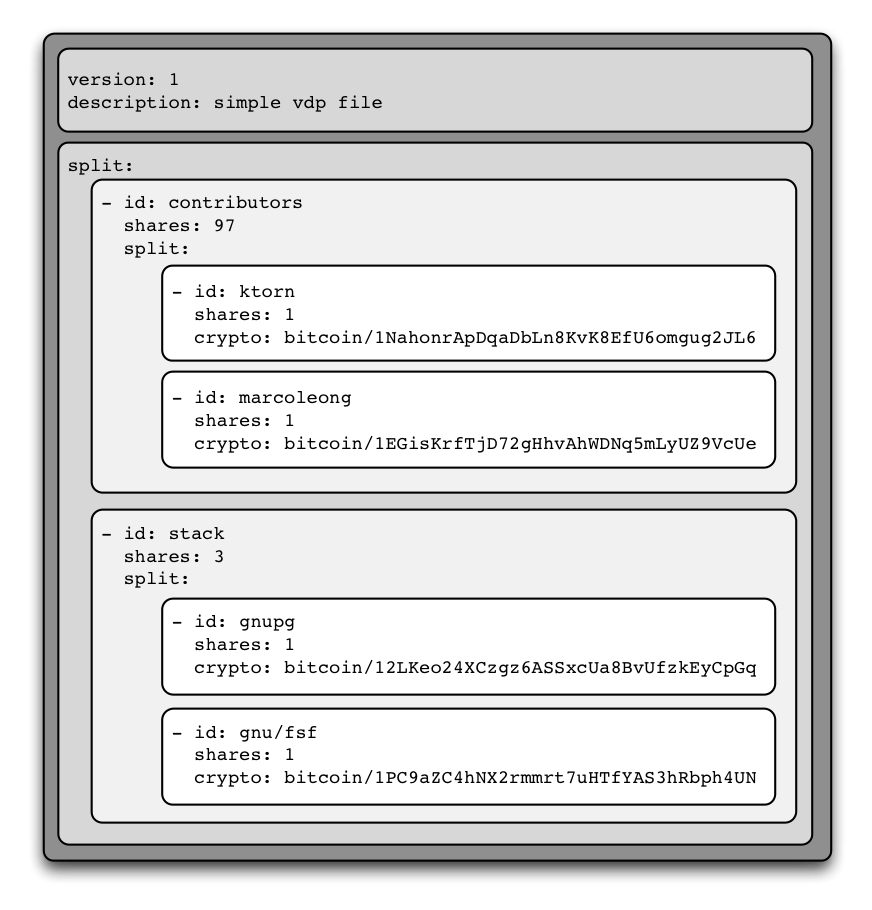
\includegraphics[width=\textwidth]{vdp-example1.png}
    \caption{Example VDP Configuration File}
    \label{fig:vdp1}
  \end{subfigure}
  \hfill
  \begin{subfigure}[b]{0.45\textwidth}
    \centering
    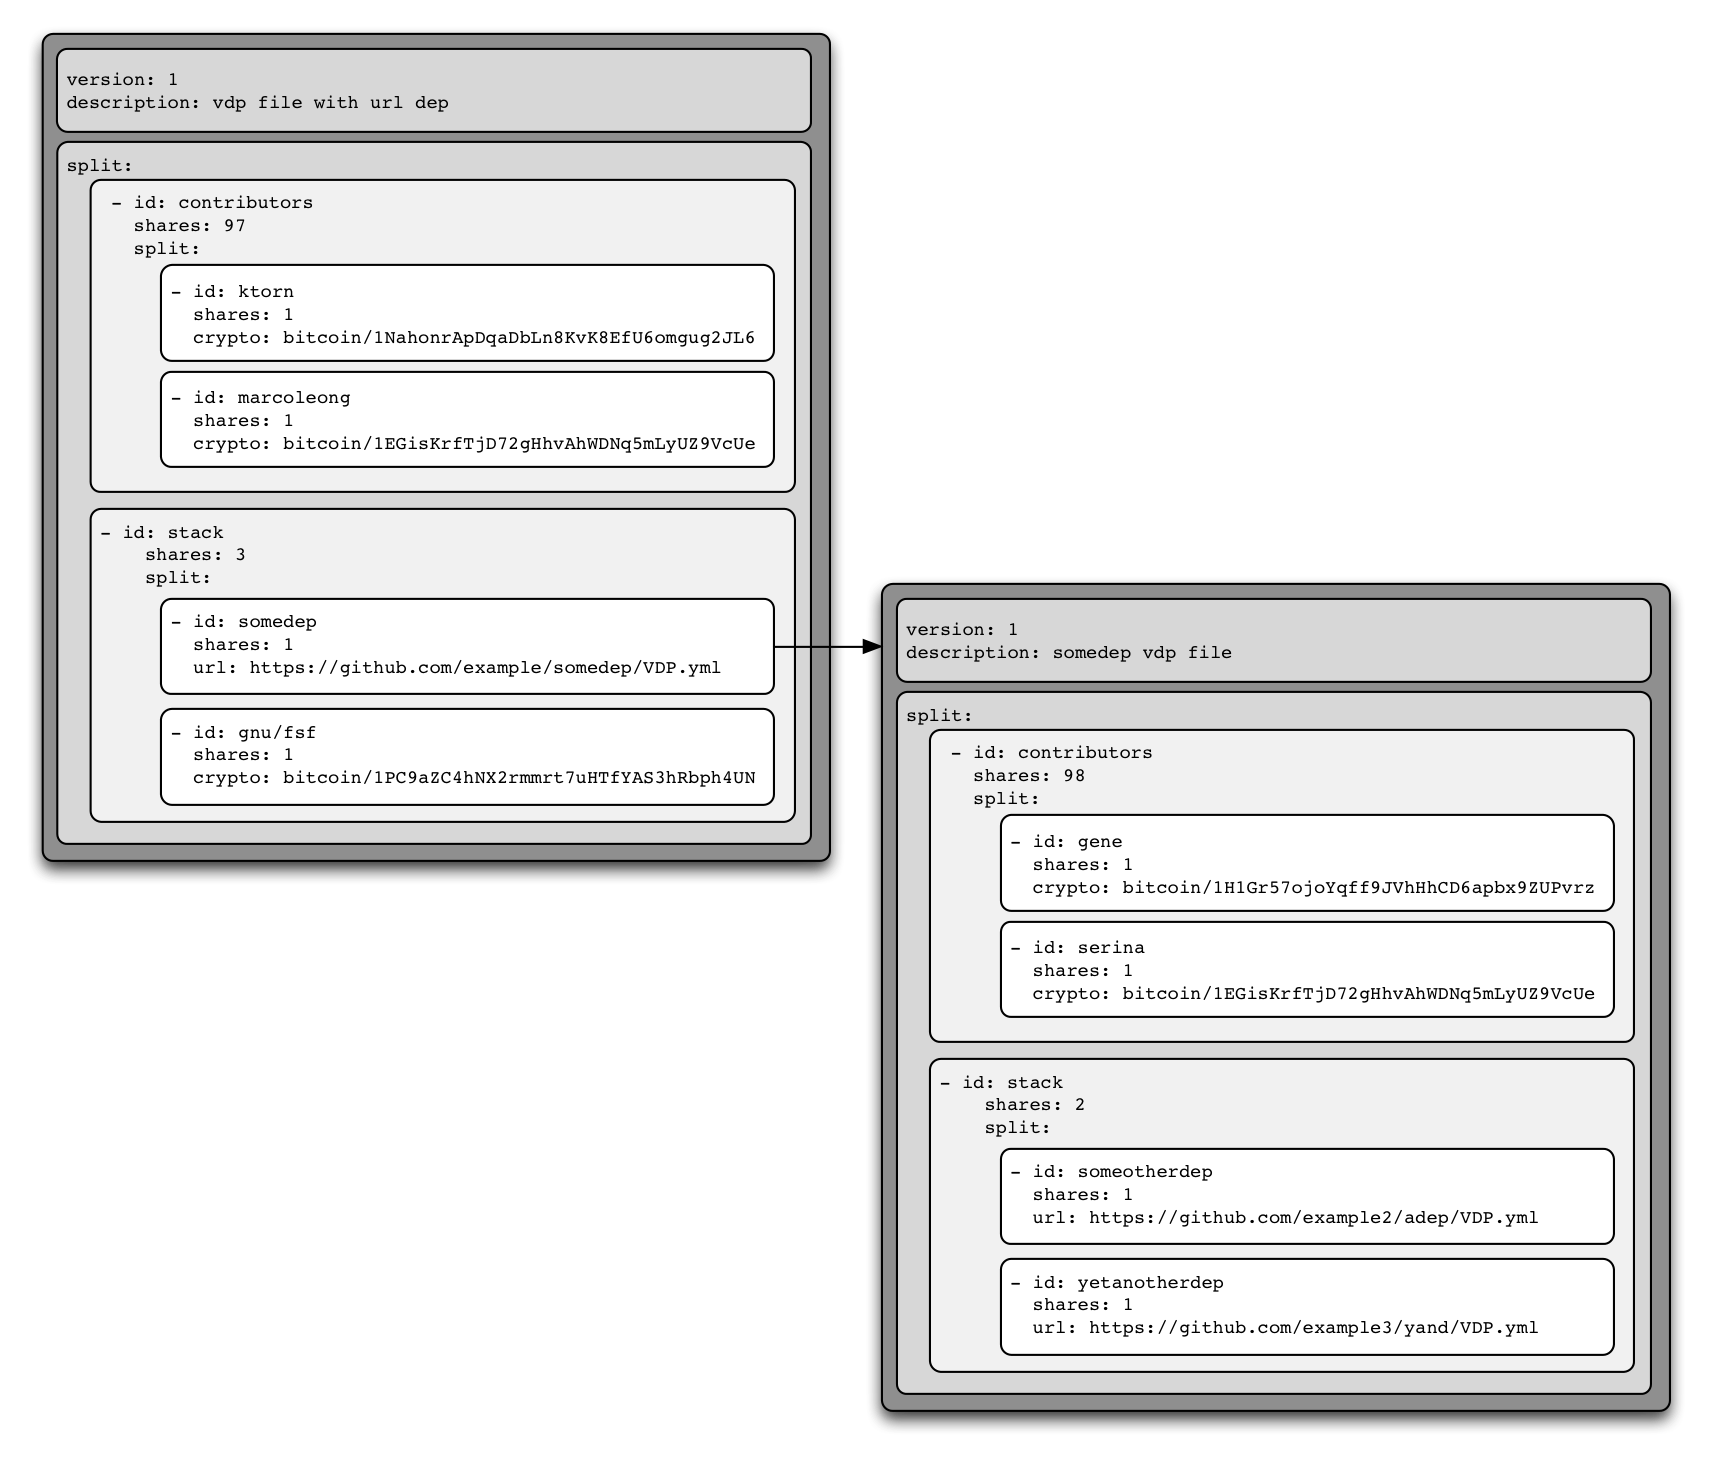
\includegraphics[width=\textwidth]{vdp-example2.png}
    \caption{Example VDP File Linking}
    \label{fig:vdp2}
  \end{subfigure}
  \caption{Example VDP Configuration Files. \\ Source: https://github.com/ktorn/vdp}
  \label{fig:vdp-examples}
\end{figure}


\begin{figure}[h]
    \centering
    \captionsetup{justification=centering}
    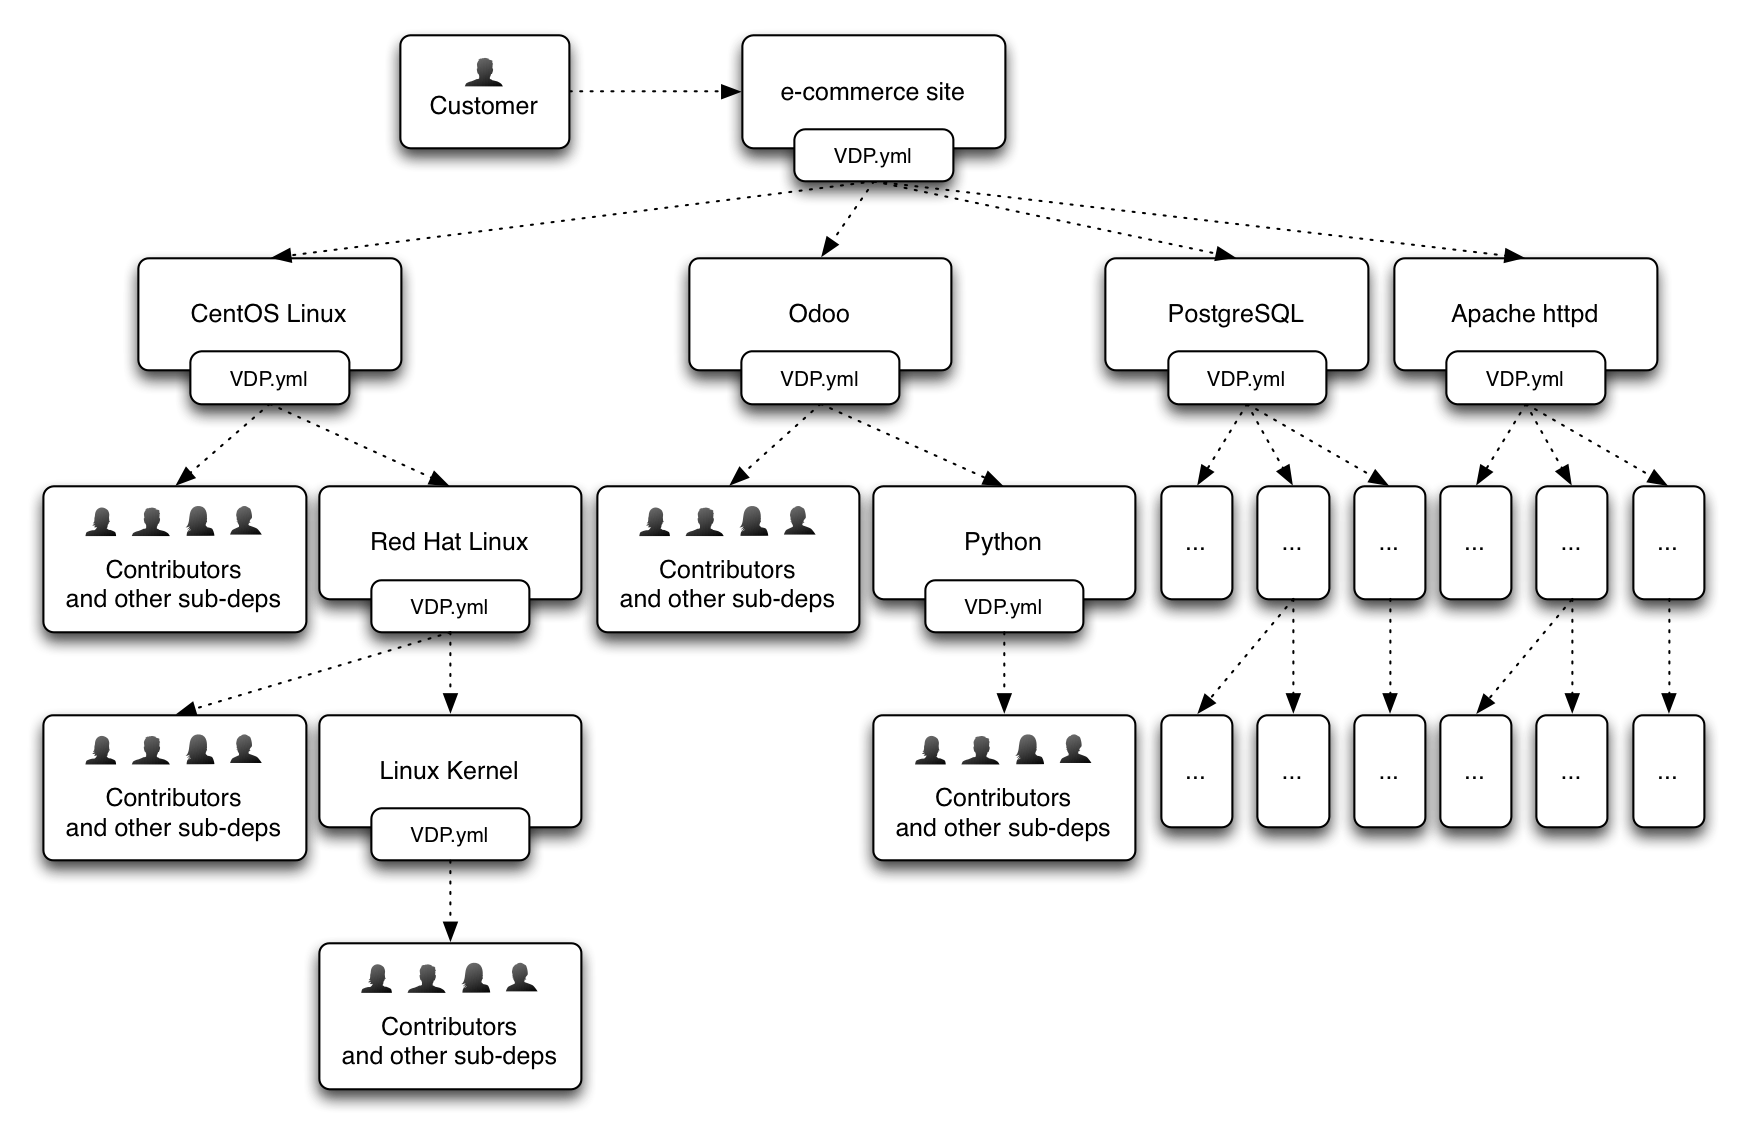
\includegraphics[width=0.75\linewidth]{vdp-opensource-usecase.png}
    \captionsetup{justification=centering}
    \caption[Value Distribution Protocol]{Value Distribution Protocol Example. \\ Source: https://github.com/ktorn/vdp}
    \label{fig:vdp}
\end{figure}

The concept is based on the idea of splitting revenue amongst stakeholders, including a small donation to project dependencies which enabled that revenue to be generated in the first place. If each project subsequently does the same, a tree of dependencies emerges, where value can flow from the top, where economic transactions are taking place, down to every dependency, and down to individual contributors. The idea was originally proposed for funding key open source projects that the Internet infrastructure depends on, but which are often forgotten about, such as OpenSSL and GPG \cite{oberhausInternetWasBuilt2019}.

This is relevant for this study since the main goal is to design and implement a sustainable artifact that can supports the long-term preservation of networked crypto art.

In this context, some progress has been made within the Tezos ecosystem, with the introduction of a collab smart contract during HEN's hicathon \cite{HicathonDocsWG2021}, a project in which the author participated, and which allows artists to not only to split royalties amongst collaborators, but also to make small donations to \emph{beneficiaries} from their art sales royalties.

In theory, if \texttt{ARKIVO} is perceived by artists as providing a useful service to networked crypto art, then by donating a small percentage of the royalties from the sales of those networked artworks to the project, then it could become economically sustainable.

\section{Teia and HEN OBJKT architecture}

In order to understand the overall structure in which OBJKTs exist, we will examine the architecture of the Teia platform.

Three main smart contracts are currently used:

\begin{itemize}
    \item HEN Minter contract: \texttt{KT1Hkg5qeNhfwpKW4fXvq7HGZB9z2EnmCCA9} 
    \item HEN FA2 Token (OBJKT): \texttt{KT1RJ6PbjHpwc3M5rw5s2Nbmefwbuwbdxton}
    \item Teia Marketplace contract: \texttt{KT1PHubm9HtyQEJ4BBpMTVomq6mhbfNZ9z5w}
\end{itemize}

When an artist mints a new OBJKT, the following takes place:

\begin{enumerate}
    \item Artist fills in artwork details in the Teia UI (including title, description, tags, number of editions, and royalties)
    \item Teia UI prepares the OBJKT metadata, and uploads it, along with the artwork's assets to IPFS, via Teia's own IPFS infrastructure
    \item Teia UI prompts user to initiate the blockchain transaction, via their Tezos wallet
    \item User's Tezos wallet calls \texttt{mint\_OBJKT} endpoint on the HEN Minter smart contract, including the metadata IPFS CID created in step 2.
    \item The HEN Minter smart contract verifies the call, and calls \texttt{mint} on the HEN OBJKT (FA2) smart contract, where the OBJKTs are actually stored
\end{enumerate}

After a few moments, the transaction confirms on the blockchain and the indexers, TzKT and Teztok, will pick up the new mint, and index it. This then allows the Teia UI to pick up the change and show the minted OBJKT to the artist. The artist will see a balance of 

At this stage the artist can list the OBJKT for sale, by making a subsequent transaction, which effectively transfers some editions from his wallet to the Teia Marketplace, where they can be collected by others for the specified price.

\begin{figure}[h]
    \centering
    \captionsetup{justification=centering}
    \includesvg[width=\textwidth]{hen-teia-components}
    \caption[Teia and HEN OBJKT architecture]{Teia and HEN OBJKT architecture}
    \label{fig:teia-arch}
\end{figure}

Once minted, an OBJKT's metadata becomes immutable. This means an OBJKT can only ever point at one CID and that cannot be changed.

\begin{figure}[h]
    \centering
    \captionsetup{justification=centering}
    \includesvg[width=\textwidth]{objkt-structure.svg}
    \caption[HEN OBJKT Structure]{HEN OBJKT Structure}
    \label{fig:objkt-struct}
\end{figure}

\subsection{OBJKT metadata}

An example OBJKT metadata is as follows:

\vspace{0.5cm}

\begin{lstlisting}[language=, caption={Example OBJKT Metadata}]
{
  "name": "This is not an evolving artwork",
  "description": "This OBJKT is only for testing purposes.",
  "tags": [
    "evolving",
    "seda"
  ],
  "symbol": "OBJKT",
  "artifactUri": "ipfs://QmbbgnKF94WowkANGrzRhJ4kZZaCjt85qC6ikW1XaaayBW",
  "displayUri": "ipfs://QmbbgnKF94WowkANGrzRhJ4kZZaCjt85qC6ikW1XaaayBW",
  "thumbnailUri": "ipfs://Qmac5jhpxNukkGm561jQN79Csp24s997PF51wvHxLKS3mz",
  "creators": [
    "tz1dd2tmTJFRJh8ycLuZeMpKLquJYkMypu2Q"
  ],
  "formats": [
    {
      "mimeType": "image/png",
      "fileSize": 1706829,
      "fileName": "not-evolving.png",
      "dimensions": {
        "value": "1024x1024",
        "unit": "px"
      },
      "uri": "ipfs://QmbbgnKF94WowkANGrzRhJ4kZZaCjt85qC6ikW1XaaayBW"
    },
    {
      "mimeType": "image/png",
      "fileSize": 256717,
      "fileName": "thumbnail_not-evolving.png",
      "dimensions": {
        "value": "350x350",
        "unit": "px"
      },
      "uri": "ipfs://Qmac5jhpxNukkGm561jQN79Csp24s997PF51wvHxLKS3mz"
    }
  ],
  "decimals": 0,
  "isBooleanAmount": false,
  "shouldPreferSymbol": false,
  "rights": "cc-by-nc-4.0",
  "date": "2024-08-26T15:13:18.882Z",
  "mintingTool": "https://teia.art/mint"
}
\end{lstlisting}

Note how how static image assets contain information about their dimensions (automatically extracted from the images by the Teia UI during the minting), however this is not the case of code-based OBJKTs (mime-type \texttt{application/x-directory}), also called \emph{Interactives} in HEN terminology, as can be seen in listing \autoref{lst:code-based-meta}:

\begin{lstlisting}[language=, caption={Excerpt from Code-Based OBJKT Metadata}, label={lst:code-based-meta}]
[snip]
"formats": [
    {
      "fileSize": 1700696,
      "fileName": "evolving-genesis-mint.zip",
      "mimeType": "application/x-directory",
      "uri": "ipfs://bafybeicx7ctb5n6bvalsdlmnsphizsopzejzw5zeqpurzu3jpkipmvxsle"
    },
    {
      "mimeType": "image/png",
      "fileSize": 1703771,
      "fileName": "cover_evolving-genesis-mint.png",
      "dimensions": {
        "value": "1024x1024",
        "unit": "px"
      },
      "uri": "ipfs://QmSHcauxV81hGvF89HF7VNXSeLpCJo4oPVSX7Gobns6Yfm"
    },
[snip]
\end{lstlisting}

This means we do not have the information about the native resolution of the code-based OBJKT at the time of minting, and this causes issues when rendering these artworks, as the size of the iframe cannot be adjusted accordingly. This is a known problem with code-based OBJKTs which will hopefully be addressed some time in the future, potentially by prompting the artist to supply that information during the minting.

\subsection{Content-Security-Policy for Interactives}

When minting a code-based (or Interactive) OBKJT via the HEN and now Teia UI, a Content-Security-Policy meta tag is injected into the OBJKT's \texttt{index.html} page. This is done by the Teia UI itself. The original intention being the restriction of network requests to a list of allowed domain names, for security purposes. However this security measure can be easily bypassed by anyone who mints an OBJKT by interacting directly with the smart contract, bypassing the Teia UI, or using a modified version of the Teia UI (which is open source).

\begin{lstlisting}[language=, caption={Content-Security-Policy meta tag added to all Interactive OBJKTs}, label={lst:code-based-meta}]
   <meta http-equiv="Content-Security-Policy" content="
    upgrade-insecure-requests;
    default-src
      'none';
    frame-src
      'self';
    child-src
      'self';
    script-src
      'self'
      'unsafe-inline'
      'unsafe-eval'
      blob:;
    style-src
      'self'
      'unsafe-inline';
    img-src
      'self'
      'unsafe-inline'
      data:
      blob:
      https://ipfs.infura.io
      https://cloudflare-ipfs.com/
      https://ipfs.io/
      https://gateway.pinata.cloud/;
    font-src
      'self'
      https://ipfs.infura.io
      https://cloudflare-ipfs.com/
      https://fonts.googleapis.com/
      https://ipfs.io/
      https://gateway.pinata.cloud/;
    connect-src
      'self'
      https://better-call.dev
      https://*.better-call.dev
      https://*.cryptonomic-infra.tech
      https://cryptonomic-infra.tech
      https://*.infura.io
      https://infura.io
      blob:
      ws:
      wss:
      bootstrap.libp2p.io
      preload.ipfs.io
      https://api.etherscan.io
      https://api.thegraph.com
      https://*.tzkt.io
      https://api.tzstats.com
      https://*.wikidata.org
      https://*.coinmarketcap.com
      https://api.openweathermap.org
      https://hicetnunc.xyz
      https://*.hicetnunc.xyz;
    manifest-src
      'self';
    base-uri
      'self';
    form-action
      'none';
    media-src
      'self'
      'unsafe-inline'
      data:
      blob:
      https://ipfs.infura.io
      https://cloudflare-ipfs.com/
      https://ipfs.io/
      https://gateway.pinata.cloud/;
    prefetch-src
      'self'
      https://ipfs.infura.io
      https://cloudflare-ipfs.com/
      https://fonts.googleapis.com/
      https://ipfs.io/
      https://gateway.pinata.cloud/;
    worker-src
      'self'
      'unsafe-inline'
      blob:;">
\end{lstlisting}


\section{Survey of Code-Based Crypto Art}
\label{sec:survey-crypto-art}

\begin{figure}[h]
    \centering
    \captionsetup{justification=centering}
    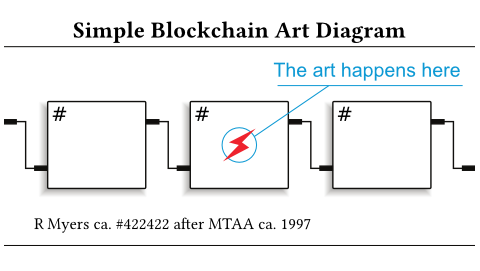
\includegraphics[width=0.50\linewidth]{simple-blockchain-art-diagram.png}
    \captionsetup{justification=centering}
    \caption[Simple Blockchain Art Diagram, by Rhea Myers]{Simple Blockchain Art Diagram, by Rhea Myers. \\ Source: https://rhea.art/simple-blockchain-art-diagram/}
    \label{fig:vdp}
\end{figure}



In the following section several code-based crypto artworks will be reviewed. They were selected for their unique properties, with the goal of providing a representative sample of the types of artworks available and helping understand the challenges that they pose from a preservation point of view.

\subsection{Configurable API Endpoints}

Stevie Jones, a.k.a. 1x1, pioneered the use of an interactive options menu which allows the user to modify the IPFS endpoint domain name, hence dealing with the mutable dependency dilemma directly on the OBJKT. However the piece also makes a request to \texttt{api.better-call.dev}, and endpoint which is not longer available. According to Stevie, the request was to check if the viewer owned 2 previous editions of the series, in which case additional content would be unlocked. From a preservation perspective, the challenge with this piece is the fact that it is fully interactive, and it requires clicking on each track to initiate the respective network request. A single automated snapshot archive of this OBJKT will be highly incomplete, as it will be missing all the media.

\begin{figure}[H]
  \centering
  \captionsetup{justification=centering}
  \begin{subfigure}[b]{0.45\textwidth}
    \centering
    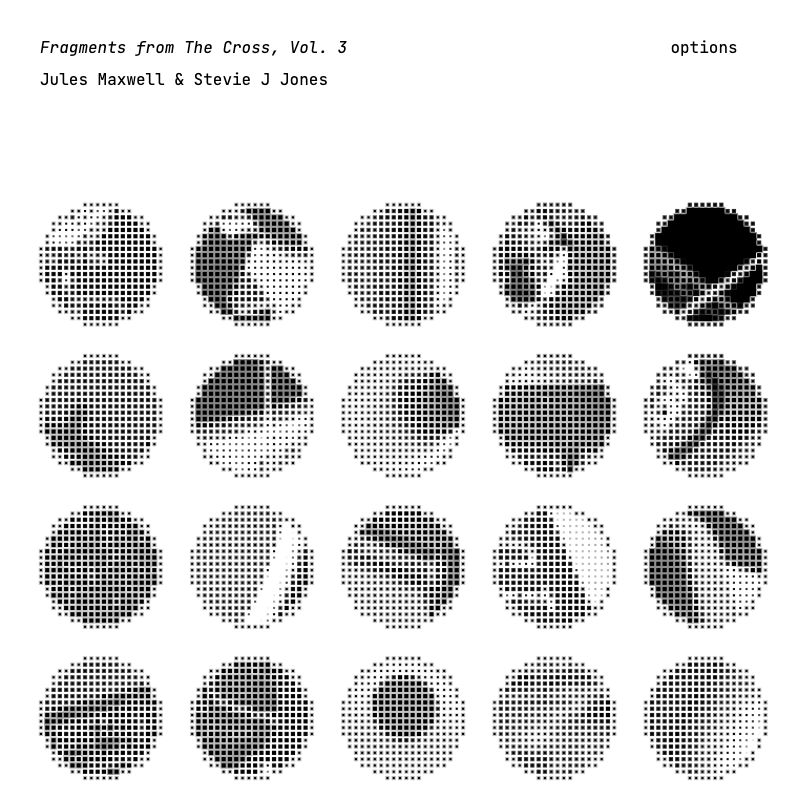
\includegraphics[width=\textwidth]{fragments-cross-main.png}
    \caption{Front Cover}
    \label{fig:vdp1}
  \end{subfigure}
  \hfill
  \begin{subfigure}[b]{0.45\textwidth}
    \centering
    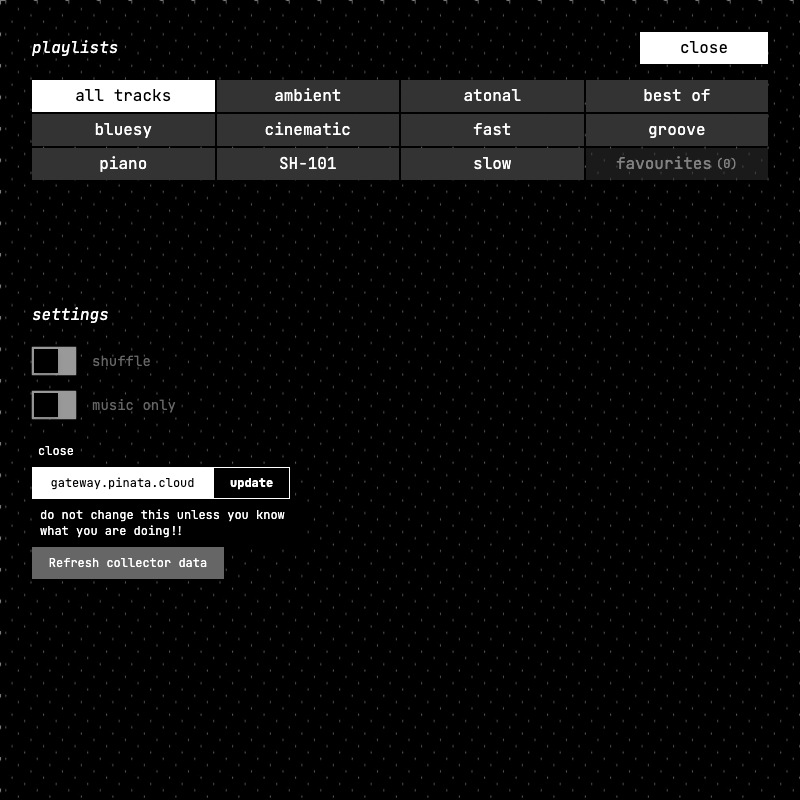
\includegraphics[width=\textwidth]{fragments-cross-menu.png}
    \caption{Options UI, with IPFS URL config}
    \label{fig:vdp2}
  \end{subfigure}
  \caption{Fragments from The Cross, Vol. 3 by Jules Maxwell \& Stevie Jones. \\ Source: https://teia.art/objkt/83079}
  \label{fig:vdp-examples}
\end{figure}


\subsection{Requests to Private Servers}

\begin{figure}[h]
    \centering
    \captionsetup{justification=centering}
    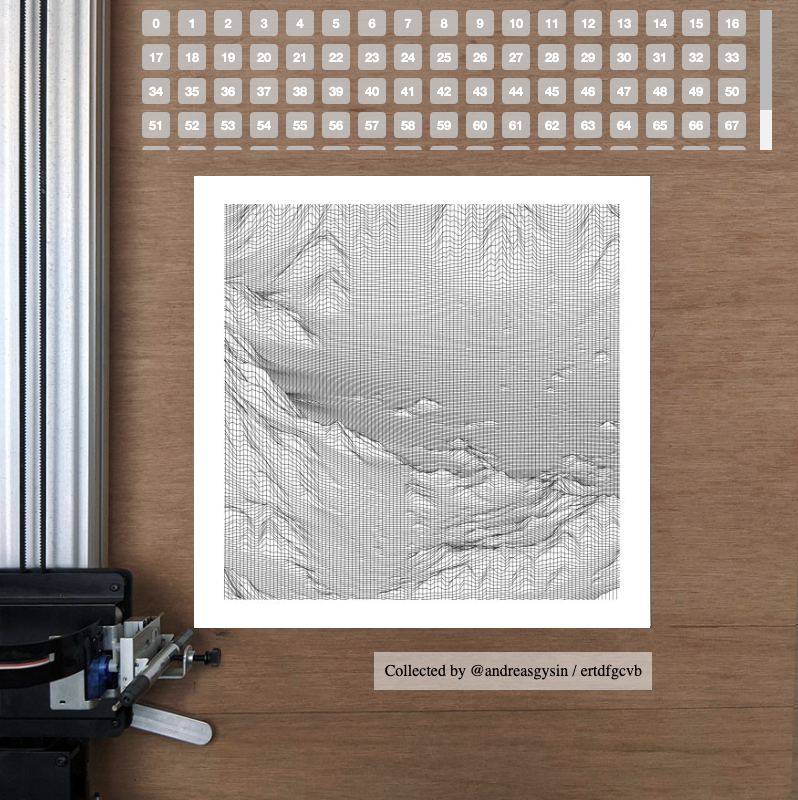
\includegraphics[width=0.75\linewidth]{possible-landscape.png}
    \captionsetup{justification=centering}
    \caption[a possible landscape by Joanie Lemercier]{a possible landscape by Joanie Lemercier. \\ Source: https://teia.art/objkt/33076}
    \label{fig:vdp}
\end{figure}

In a groundbreaking conceptual piece within the context of HEN, Joanie Lemercier, linked the act of collecting the piece with the drawing of a physical plotter landscape, which would be revealed within the OBJKT itself. Minted at a time when there were no restrictions on network request destinations, Lemercier uses requests to his own personal domain, \texttt{https://joanielemercier.com}, to load the assets for each print completed. Similarly to Stevie's Fragments of a Cross, it only initiates these requests when a user interacts with the piece.

Since, according to Lemercier, this piece is now ``completed'', one single full snapshot, including the recording/archival of each and every landscape would suffice. This is is an important intervention as the assets in the private server are a much higher risk than assets stored in IPFS.

\begin{figure}[h]
    \centering
    \captionsetup{justification=centering}
    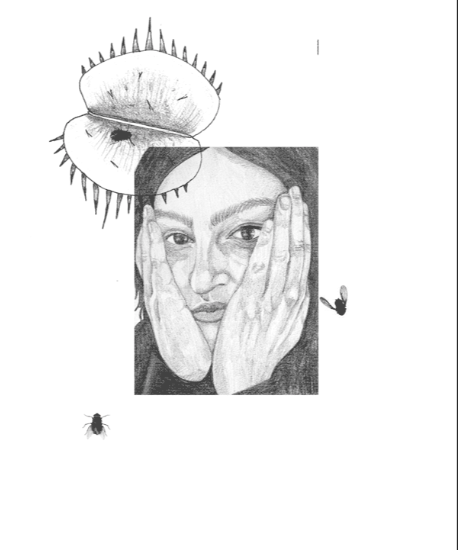
\includegraphics[width=0.50\linewidth]{becoming-body.png}
    \captionsetup{justification=centering}
    \caption[Becoming-body by Jessica Luz and Carlos de Oliveira Junior]{Becoming-body by Jessica Luz and Carlos de Oliveira Junior. \\ Source: https://teia.art/objkt/168794}
    \label{fig:becoming-body}
\end{figure}

\subsection{Requests to Indexers}

Several networked HEN OBJKTs made use of requests to indexers, to retrieve the list of collectors, amount spent on the artwork, and other blockchain or market related data.
We already mentioned ``Planned Obsolescence'' by Mario Klingemann, see page \pageref{fig:plannedobsolescence}.

``Becoming-body'', a collab between Brazillian artists Jessica Luz and Carlos de Oliveira Junior (a.k.a. @vamoss), was created within the TIBUM residency. The artwork contains a series of 36 animated GIFs, which will swap each time the artwork is collected, see \autoref{fig:becoming-body}.


\subsection{Requests to RPC nodes}

Yazid, one of the most prolific author of networked OBJKTs on HEN, in ``OBJKTs (Mondrian Edition)'' ditched the dependency on indexers in favour of embedding the Taquito JS library, which enabled the piece to contact the RPC nodes directly. In addition to cycling through 2 RPC endpoints for extra resiliency, the RCP API is also more stable than indexer APIs. A testament to this resiliency is the fact that this OBJKT still works today. The OBJKT queries the blockchain every minute for the latest OBJKT ID minted, and represents it as a series of bars in a Mondrian style, each column representing a digit of the number. See \autoref{fig:mondrian}. This means the artwork evolves rather quickly, with the rendering changing each time another OBJKT gets minted, in real time.

\begin{figure}[h]
    \centering
    \captionsetup{justification=centering}
    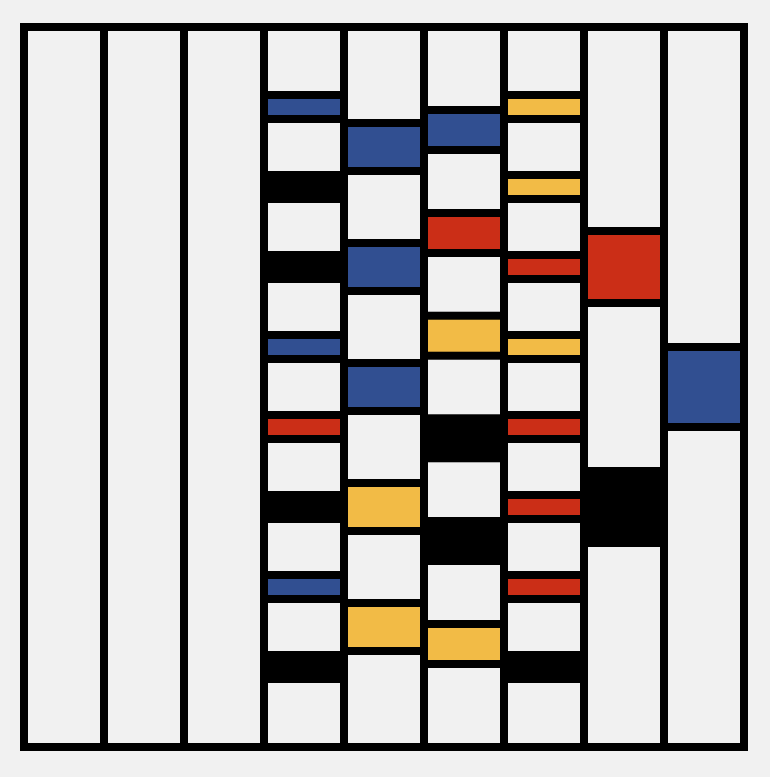
\includegraphics[width=0.50\linewidth]{objkts-mondrian.png}
    \captionsetup{justification=centering}
    \caption[OBJKTs (Mondrian Edition) by Yazid]{OBJKTs (Mondrian Edition) by Yazid. \\ Source: https://arkivo.art/artifacts/HEN/200599}
    \label{fig:mondrian}
\end{figure}

London-based James Bloom is another artist known for his blockchain-interactive artworks. Using a mixture of requests to configurable RPC endpoints and private infrastructure, James creates artworks that react in real-time to changes in the blockchain, Ethereum in this case. Mass is particularly interesting because the artwork monitors every action its owners take on-chain, and uses that data to enact changes in the rendered 3D space, in what James calls a "mass surveillance machine".

\begin{figure}[h]
    \centering
    \captionsetup{justification=centering}
    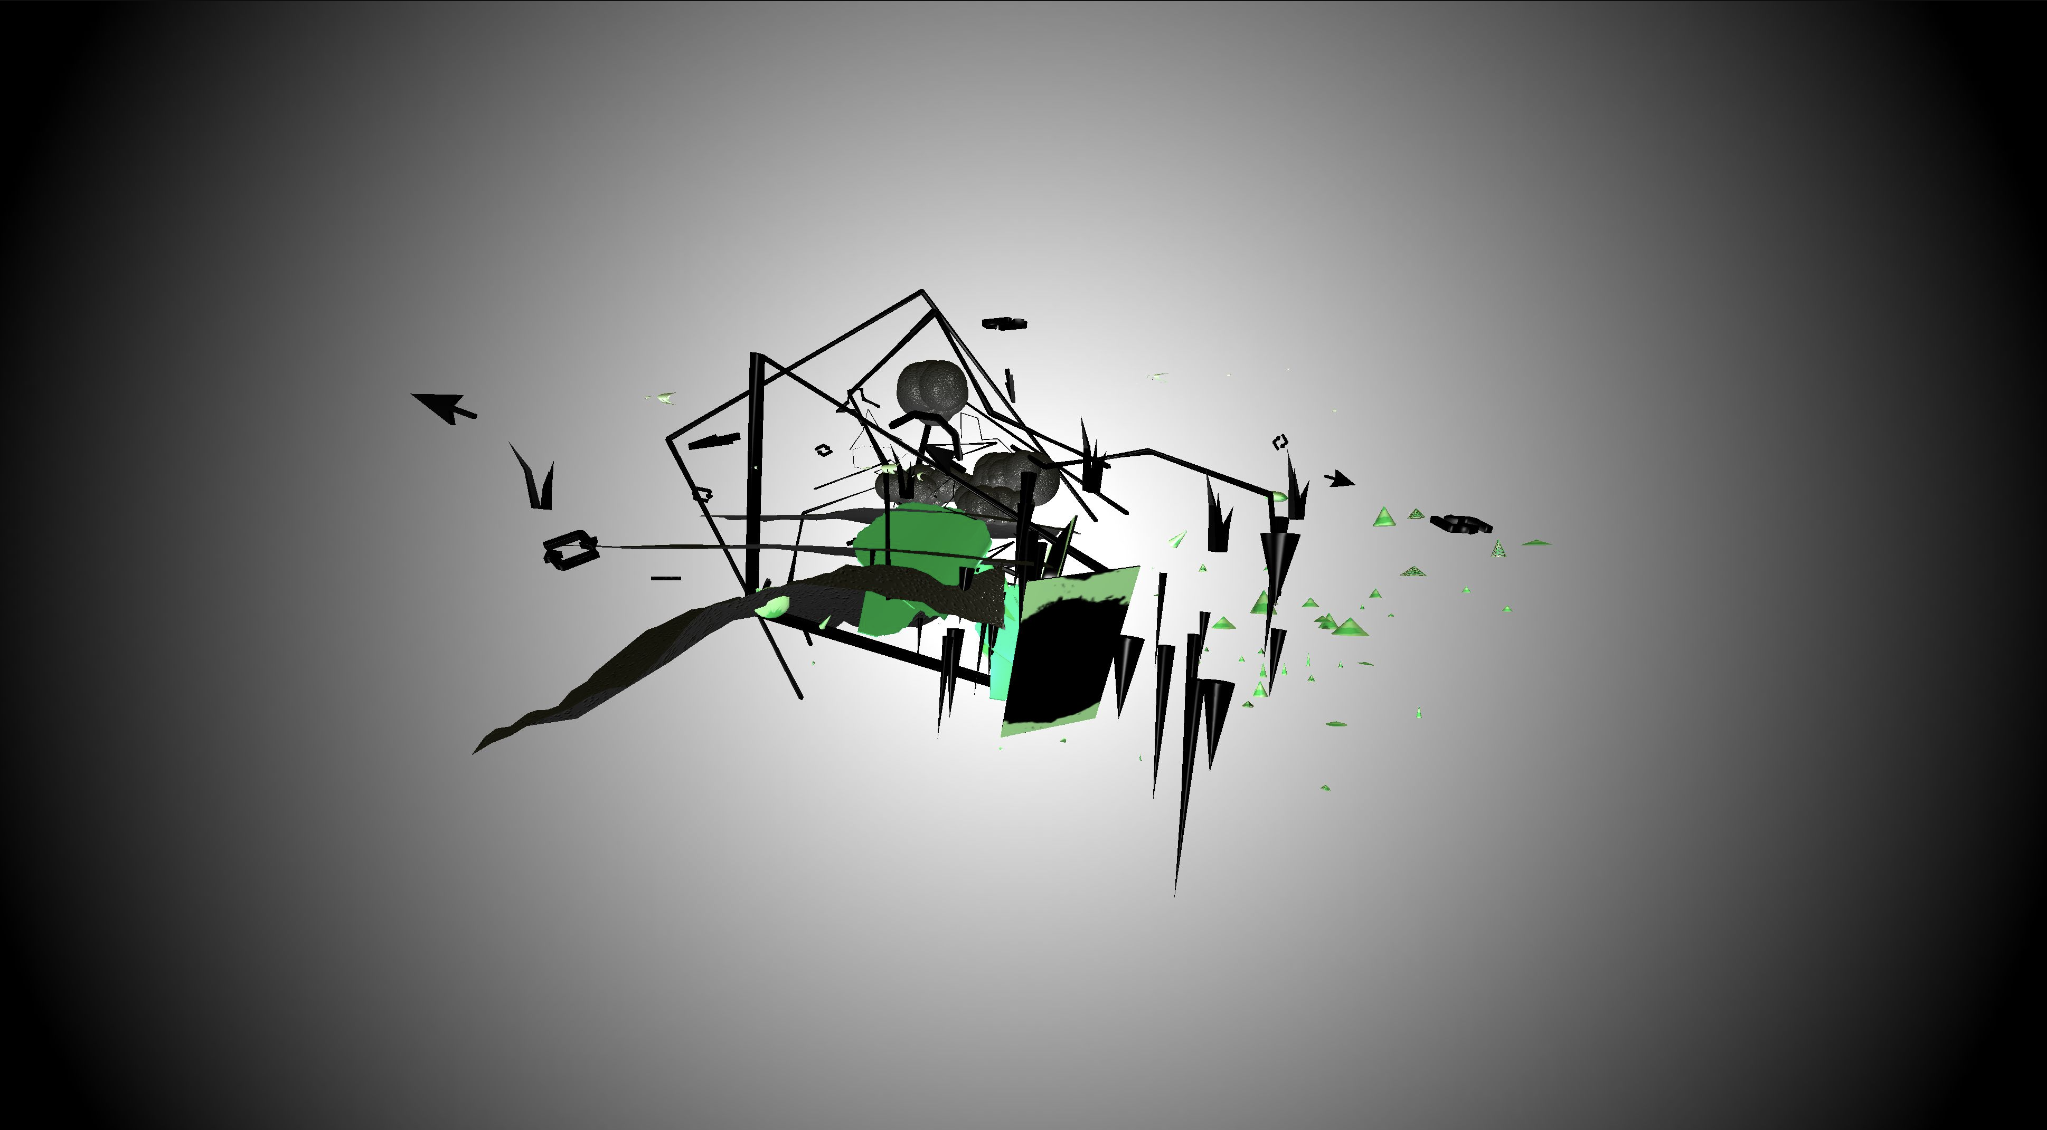
\includegraphics[width=0.75\linewidth]{mass.png}
    \captionsetup{justification=centering}
    \caption[Mass \#1 by James Bloom]{Mass \#1 by James Bloom. \\ Source: https://opensea.io/assets/ethereum/ \\
    0x80faa45d6f6cbdafdeba2f9c4a0237f74e5d8d9c/1}
    \label{fig:mass}
\end{figure}


\subsection{Custom Renderings Based on Ownership}

Another common theme amongst code-based OBJKTs is the customisation of the rendering based on whether the viewer owns the artwork. The piece can tell the Tezos wallet address of the viewer because, if the user is logged in to Teia, it passes their wallet address to piece via URL query parameters. The piece then can query the blockchain to determine if that address owns any editions of itself, or even of other OBJKTs.

Raphaël de Courville has experimented with this idea in two conceptual artworks. The first one, Adam, consults the blockchain (via the hicdex indexer) and gathers how many editions of the artwork have been sold, data which it uses to start erasing itself gradually. However at the same time it also checks how many editions of the artwork the viewer owns, and modifies the rendering slightly for them. These changes are subtle, resulting in a slow evolution over time.

\begin{figure}[h]
    \centering
    \captionsetup{justification=centering}
    \fcolorbox{gray}{white}{
\includegraphics[width=0.50\linewidth]{adam-full.png}}
    \captionsetup{justification=centering}
    \caption[Adam by Raphaël de Courville (sableraph)]{Adam by Raphaël de Courville (sableraph). \\ Source: https://teia.art/objkt/230177}
    \label{fig:mondrian}
\end{figure}


\begin{figure}[H]
  \centering
  \captionsetup{justification=centering}
  \begin{subfigure}[b]{0.45\textwidth}
    \centering
    \fcolorbox{gray}{white}{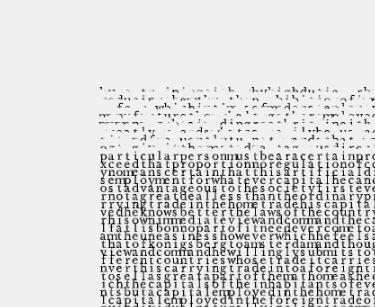
\includegraphics[width=\textwidth]{adam-no-own.png}}
    \caption{Viewer does not own OBJKT}
    \label{fig:adam-no-own}
  \end{subfigure}
  \hfill
  \begin{subfigure}[b]{0.45\textwidth}
    \centering
    \fcolorbox{gray}{white}{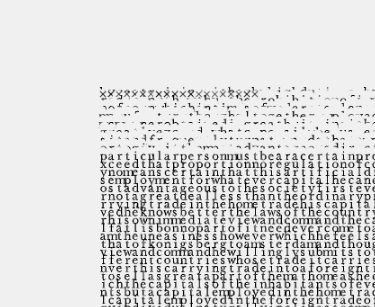
\includegraphics[width=\textwidth]{adam-own.png}}
    \caption{Viewer owns 5 editions of OBJKT}
    \label{fig:adam-own}
  \end{subfigure}
  \caption{Detail of Adam by Raphaël de Courville (sableraph). \\ Source: https://teia.art/objkt/230177}
  \label{fig:vdp-examples}
\end{figure}

The second, a collab with Malaysian artist Mumu, ``Moon's medication : Your meditation'', explores the relationships between 2 OBJKTs. Instead of changing itself based on the number of editions that the viewer has of this OBJKT, it checks how many editions the viewer collected of another OBJKT, ``Moon's medication - Day'', and starts adding coloured medication tabs, with the amount of colours reflecting the number of editions the viewer owns: red, orange, yellow, green, blue and purple.

\begin{figure}[H]
  \centering
  \captionsetup{justification=centering}
  \begin{subfigure}[b]{0.45\textwidth}
    \centering
    \fcolorbox{gray}{white}{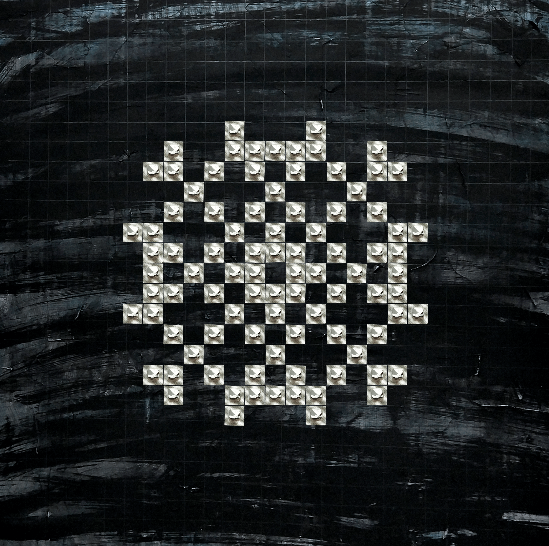
\includegraphics[width=\textwidth]{moons-med-no-own.png}}
    \caption{Viewer does not own Moon's medication - Day}
    \label{fig:adam-no-own}
  \end{subfigure}
  \hfill
  \begin{subfigure}[b]{0.45\textwidth}
    \centering
    \fcolorbox{gray}{white}{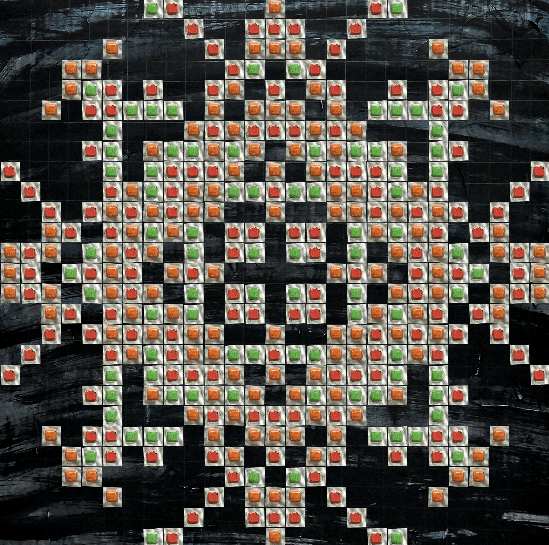
\includegraphics[width=\textwidth]{moons-med-own.png}}
    \caption{Viewer owns 3 editions of Moon's medication - Day}
    \label{fig:adam-own}
  \end{subfigure}
  \caption{Moon's medication : Your meditation by Raphaël de Courville (sableraph) and Mumu. \\ Source: https://teia.art/objkt/631387}
  \label{fig:vdp-examples}
\end{figure}


\subsection{Time/System Clock Based}

\begin{figure}[h]
    \centering
    \captionsetup{justification=centering}
    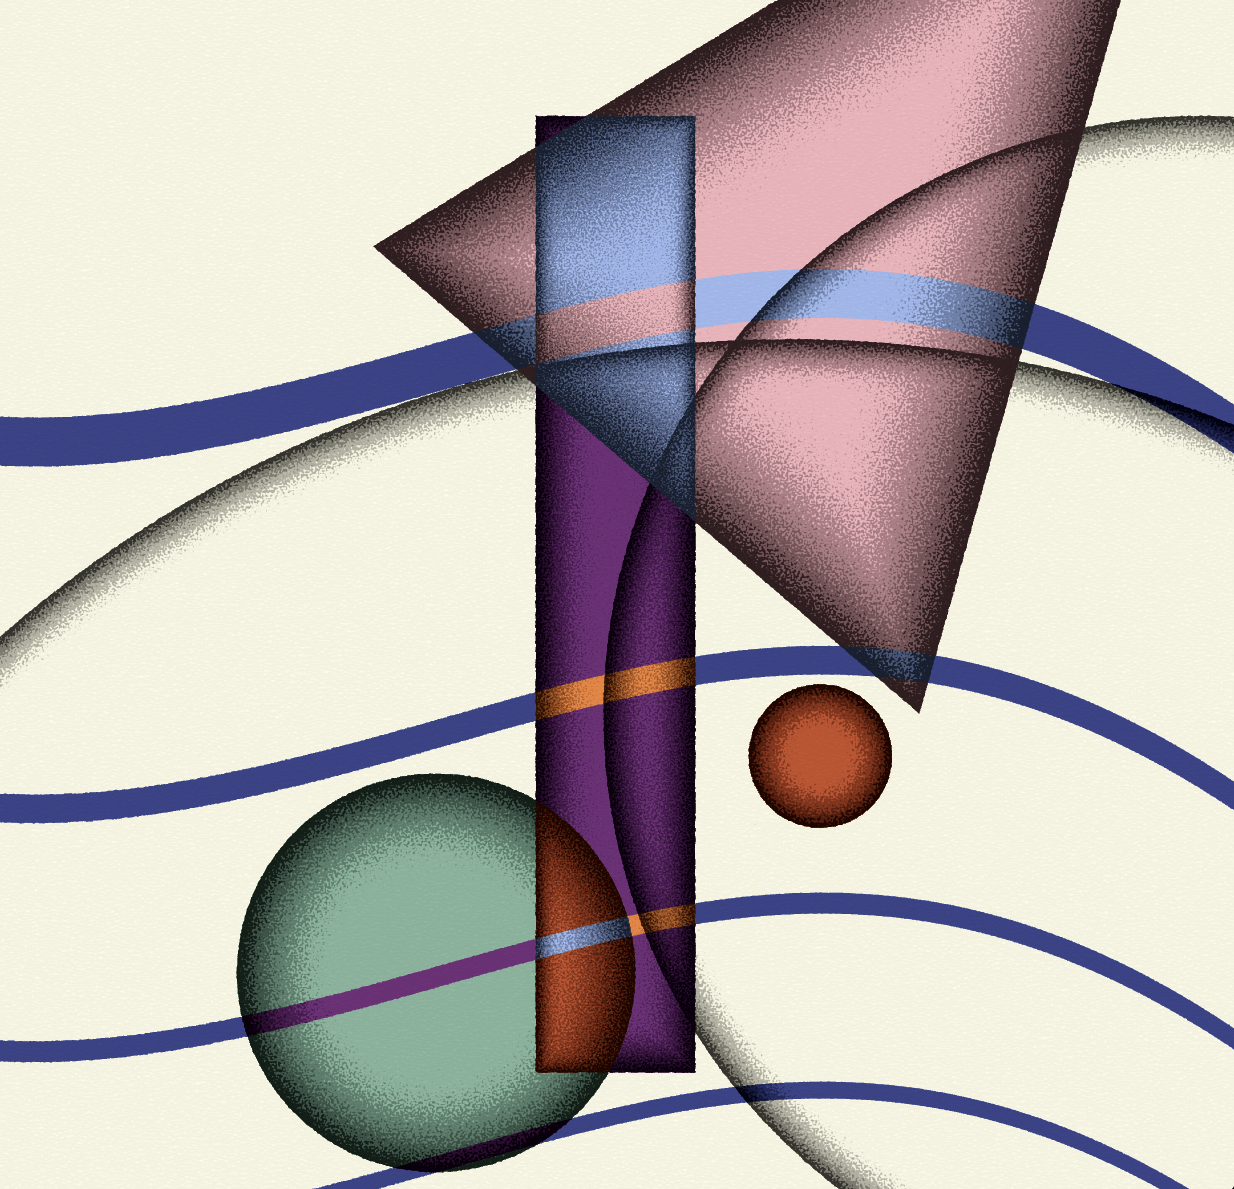
\includegraphics[width=0.50\linewidth]{detachment.png}
    \captionsetup{justification=centering}
    \caption[Detachment by Thomas Lin Pedersen]{Detachment by Thomas Lin Pedersen. \\ Source: https://thomaslinpedersen.art/work/detachment/}
    \label{fig:detachment}
\end{figure}

Code-based artworks that evolve deterministically, based purely on the system clock, have a very interesting preservation property: their complete evolution, which in theory can span thousands of years, is entirely encapsulated and self-contained in the code. Since all you need to provide the artwork with is the system time, you can in theory rewind or fast-forward hours, days, weeks, or centuries in an instant. If there was ever an artwork that encapsulates the philosophical concept of determinism, then Detachment by Thomas Lin Pedersen is a good candidate, see \autoref{fig:detachment}. The artwork is in perpetual motion. It is a slow motion, and one that is deterministically tied to the current time.
Another interesting property of this kind of artwork is that any two viewers who open the artwork at the same time, as long as their device clocks are synchronised, will visualise the exact same rendering, even across different timezones (the artwork uses UTC).

One can theorise that time-based artworks are, in fact, networked. However, instead of initiating a network request to an external API, they simply consult the API locally, which in JavaScript is as simple as: \texttt{new Date()}. The computer system in turn keeps that ``data source'' (the system clock) up-to-date by using external time servers (NTP), which keep the computers and other devices synchronised across the world.

Having said that, as tempting as it is to classify time-based artworks as networked, the fact is that they have very different conservation needs from the other kind of networked artwork that we examined before.


\subsection{Browser LocalStorage Interaction}

Several code-based artworks interact with the Browser's LocalStorage system, normally to persist configuration options. However Bjørn Staal adopted this LocalStorage as an art medium, and produced Entangled. This remarkable artwork consists of a collection of 512 editions, minted on Ethereum (256 editions) and Tezos (256 editions) throught the fxhash platform. Each of the editions is randomly paired with another across the two blockchains, and when one of these pairs are opened on the same browser instance (as small floating windows on the same web page) they interact with each other, using the LocalStorage as a way to coordinate their relative X,Y positions on the screen.

\begin{figure}[h]
    \centering
    \captionsetup{justification=centering}
    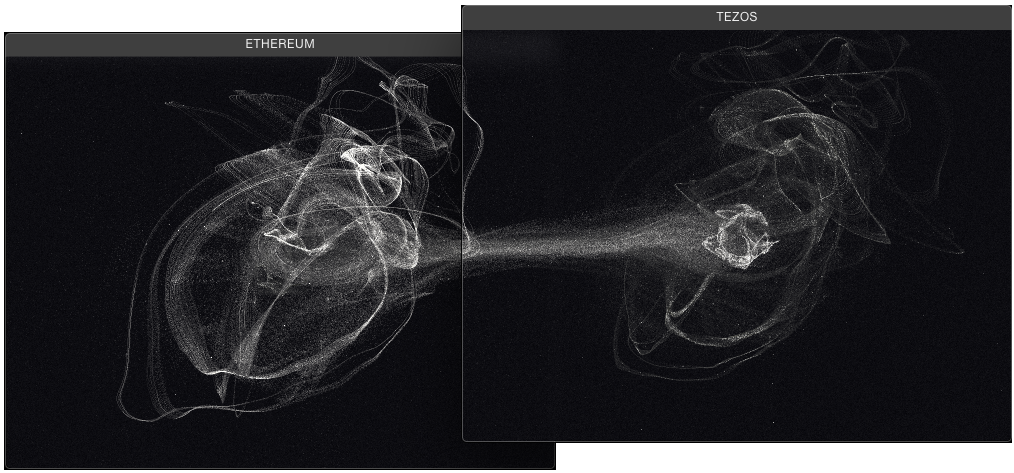
\includegraphics[width=0.75\linewidth]{entangled.png}
    \captionsetup{justification=centering}
    \caption[Entangled by Bjørn Staal]{Entangled by Bjørn Staal. \\ Source: https://www.fxhash.xyz/vertex/entangled}
    \label{fig:detachment}
\end{figure}


\subsection{Self-Contained Data}

All code-based artworks are in a way, data-driven. However all of the artwork types presented above require interacting with an external system for gaining access to that data, even if indirectly as is the case of the time-based artwork.

Javier Gracia Carpio created several data-driven artworks that package their data with the artwork's assets, therefore reducing it's dependency on external APIs. This does mean the artwork's evolution is limited to the data available to it at the time of minting. The benefit is that it makes for a very resilient artwork, with very simple preservation requirements. One such example is ``50461 users in hic et nunc'' which draws from a wide range of market activity to represent connections between users of HEN. It should be noted that this artwork is user-interactive, which does increase the complexity of preservation.

\begin{figure}[H]
    \centering
    \captionsetup{justification=centering}
    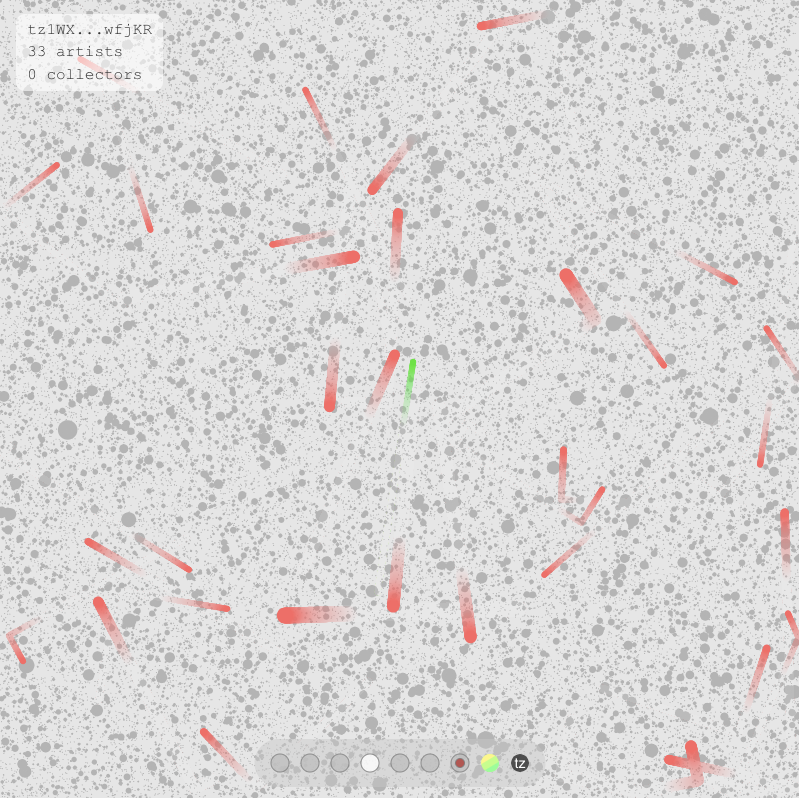
\includegraphics[width=0.50\linewidth]{hen-users.png}
    \captionsetup{justification=centering}
    \caption[50461 users in hic et nunc by Javier Gracia Carpio]{50461 users in hic et nunc by Javier Gracia Carpio. \\ Source: https://teia.art/objkt/427089}
    \label{fig:hen-users}
\end{figure}


\subsection{Determinism}

This section deals with whether artworks are deterministic in the way they are rendered or whether there is an element of randomness that even given all the same starting conditions, the artwork will look very different each time. This categorisation is important for conservation because a nondeterministic artwork will be difficult to monitor from a browser obsolescence point of view, especially when using image difference between consecutive snapshots of the artwork. In the case of a non-deterministic artwork, the snapshots will be so different that they become ineffective in detecting changes due to browser version upgrades or other changes in web specifications overtime. In this context, the challenge is to differentiate between a deterministic animated artwork, and a nondeterministic artwork. This challenge exists, because even if an artwork is deterministic, unless there is a way to snapshot the exact same frame across all the snapshots then any image difference comparisons will result in exaggerated differences. In this case we may need to employ more advanced animation frame comparison algorithms, such that the sequence of the animation can be compared across snapshots, and these may involve the recording of the animation, rather than just taking a single snapshot in time. Of course, such a strategy has trade-offs, and in this particular case the trade-off would be a much larger snapshot file size, which will then impact on the overall economic sustainability of the archive.

An example of non-deterministic artwork is Entropic, by generative art coding group united(fx). Each time the generative artwork is refreshed, a new random seed is used, resulting in a completely different output, see \autoref{fig:entropic}.

\begin{figure}[h]
    \centering
    \captionsetup{justification=centering}
    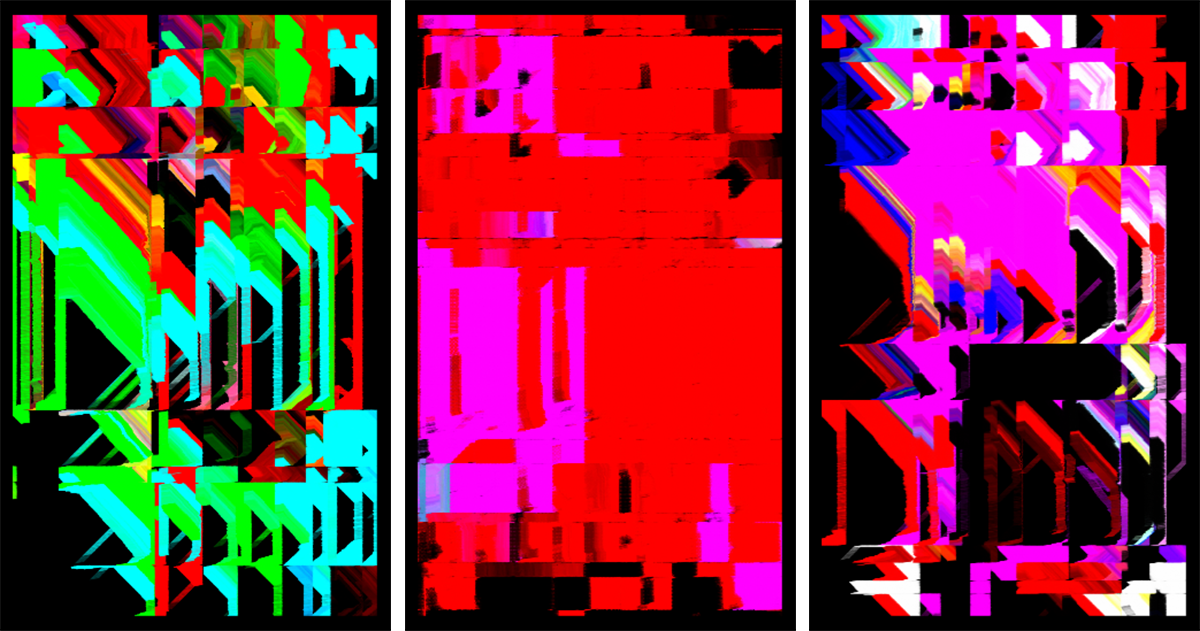
\includegraphics[width=0.75\linewidth]{entropic.png}
    \captionsetup{justification=centering}
    \caption[Entropic by united(fx) - 3 Renderings]{Entropic by united(fx) - 3 Renderings. \\ Source: https://teia.art/objkt/853589}
    \label{fig:entropic}
\end{figure}


It should be noted that, determinism is also a reason why fxhash moderates any networked NFT minted on their platform. For example, Australian artist AliaK saw her networked data-driven artwork ``data as landscape'' moderated for this reason, see \autoref{fig:aliak-data-as-landscape}.

\begin{figure}[h]
    \centering
    \captionsetup{justification=centering}
    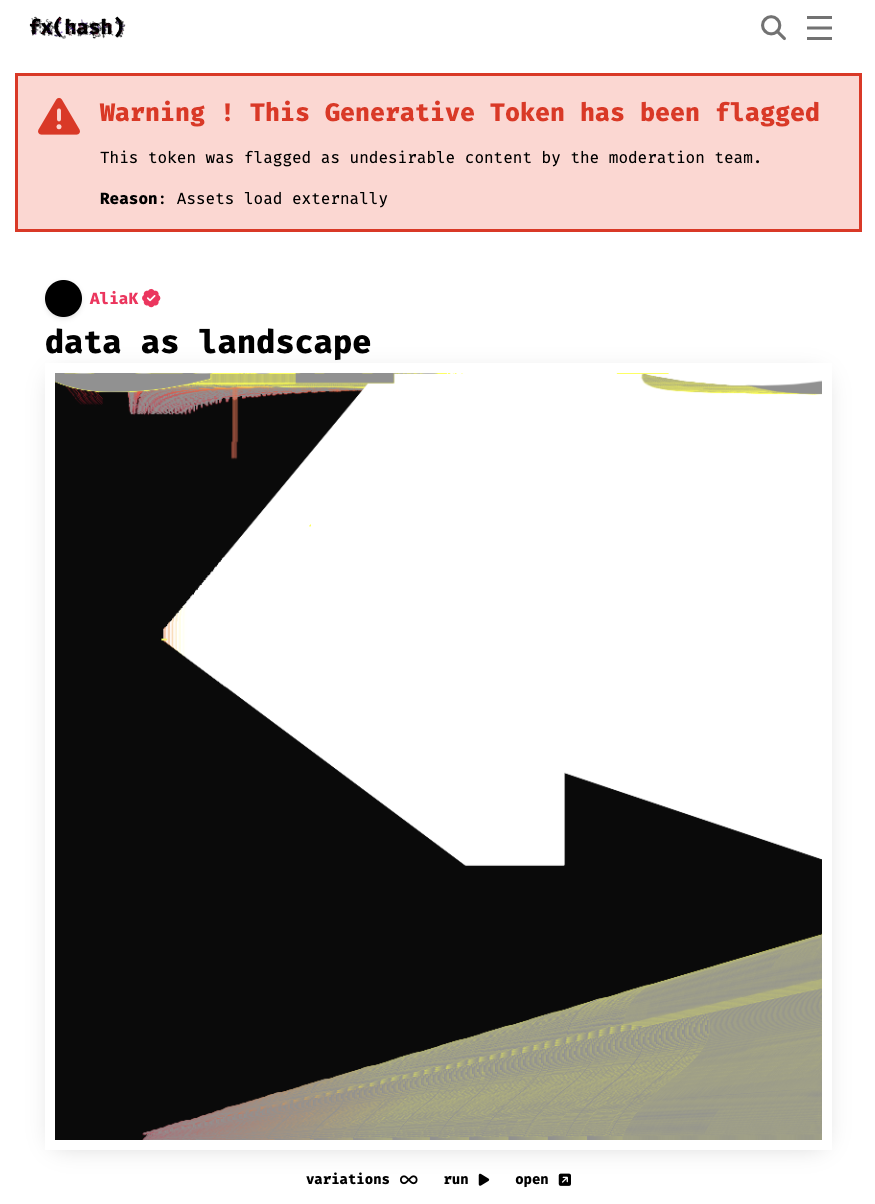
\includegraphics[width=0.5\linewidth]{aliak-data-as-landscape.png}
    \caption[Data as Landscape by AliaK]{Data as Landscape by AliaK, 2022. Source: https://www.fxhash.xyz/generative/13124}
    \label{fig:aliak-data-as-landscape}
\end{figure}



\section{Tentative Taxonomy of Code-Based Crypto Art}
\label{sec:interactivity}

When looking at the preservation of code-based crypto art, it is useful to be able to classify each artwork according to a taxonomy that informs conservators of the specific conservation methods that may be required at a later stage.

There is a clear lack of such a taxonomy in academic literature. Members of the crypto community have started efforts to classify code-based crypto art, such as Chainleft, see \autoref{fig:onchainruntimeart}.

\begin{figure}[h]
    \centering
    \captionsetup{justification=centering}
    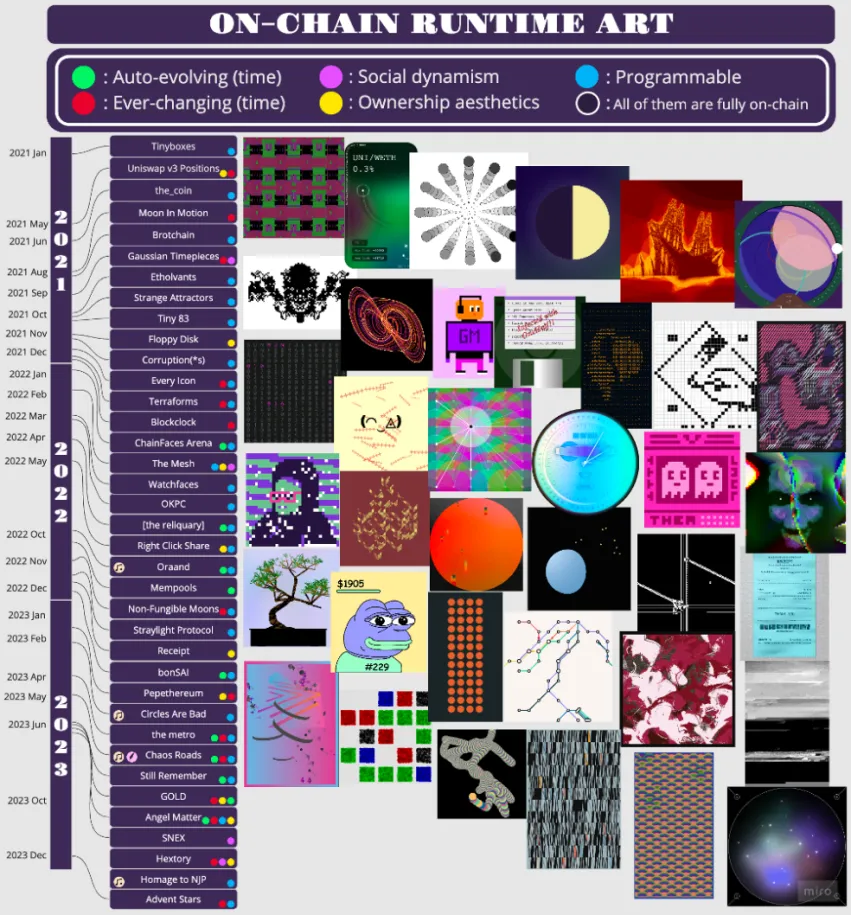
\includegraphics[width=0.75\linewidth]{chainleft-taxonomy.png}
    \caption[Onchain Runtime Art]{Onchain Runtime Art by @chainleft. Source: https://x.com/ChainLeftist/status/1757802497626767455}
    \label{fig:onchainruntimeart}
\end{figure}

Chainleft kindly shared a more detailed description of each category by private message, which can be found in \nameref{appx:chainleft-taxonomy}, page \pageref{appx:chainleft-taxonomy}. This is a good starting point for developing a taxonomy, however this study requires more fine-grained categorisation for certain technical elements of an artwork. 

For this study we will start by proposing that all code-based art is, fundamentally, data-driven. This may fall outside the traditional idea of data-driven art, which more often linked with data visualisations. The fact is that no code may run without the use of data stored in variables, and these variables maintain the internal state of the artwork. The artwork's visual rendering is only possible by materialising this internal state into visual elements on the canvas. The question then is how that data originates and which interactions cause it to change in a way that justifies capturing it from a preservation perspective.


\begin{figure}[h]
    \centering
    \captionsetup{justification=centering}
    \includesvg[width=\textwidth]{code-based-art-interaction.svg}
    \caption[Code-Based Art Interaction Channels]{Code-Based Art Interaction Channels}
    \label{fig:code-based-art-interactions}
\end{figure}

\subsection{User Interaction}

The most common kind of interaction is user interaction, through the canvas and the usual input devices. This interaction may cause the artwork to change significantly from an aesthetic perspective, but it's a private experience between the user and the artwork. It is also more than likely an ephemeral interaction, without long-lasting effects on the artwork's state. As soon as the user closes the page or browser, the changes to the artwork's state are gone, and next time the user opens the artwork, it is back to its original state. The only exception to this is if the artwork saves state on the browser's LocalStorage or IndexedDB, causing it to persist between browsing sessions. Even then, this interaction is personal to the user, and does not affect the state of the artwork for other users.

The implications of this for preservation is that the recording of a user-interactive artwork should be orchestrated to also capture some of those interactions. This is a complex task to automate.

\subsection{Time Interaction}

As mentioned above, time or system clock interaction is the easiest to capture, because all the that conservator or capturing tool need are the original artwork's assets. Then it is just a matter of manipulating the time supplied to the artwork to capture the piece in its entirety.

\subsection{Other In-Browser Interactions}

Similarly to user interaction, other modes of interaction within the browser really depend on each case. An artwork might make use of LocalStorage for enabling the interaction of two distinct tokens, as Staal did with Entangled, and in such a case the recording and documenting of such an artwork in its entirety, would be fairly complex, with so many permutations to consider.

\subsection{Network Interaction}

This study is primarily concerned with network interaction of code-based crypto artwork, because it can constitute both a persistent and an evolving state of the artwork. If an artwork deterministically gen	erates an output based on this external state, then it can be said that the network \emph{is} a part of the artwork, and needs to be captured for preservation purposes as well.

I should be noted that if the data source is the blockchain then, due to its immutable history, the full evolution of the artwork may be reconstructed in a simulation, by \emph{re-playing} the historical blockchain transactions and events required by the artwork.

However, other data sources that do not benefit for that immutable record, and of the highest concern. Fortunately, from a preservation perspective,  during the survey of artworks none have been found that rely on public, non-blockchain related, APIs.

\clearpage

Taking all the major themes from the review of the related work, as well as the survey of code-based crypto art, the following taxonomy provides a good lens through which to analyse and classify code-based crypto art.

\begin{figure}[h]
    \centering
    \captionsetup{justification=centering}
    \includesvg[width=\textwidth]{cryptoart-taxonomy.svg}
    \caption[Proposed Crypto Art Taxonomy]{Proposed Crypto Art Taxonomy}
    \label{fig:cryptoart-taxonomy}
\end{figure}

It is unfeasible to automate the classification of crypto art for all these categories at this point in time, but as we will see in \autoref{chap:dev}, we can automate two of them: code-based, and network interactive.

\section{Conclusion}

This chapter provided a review of theory of digital art conservation, and reviewed the main archival standards and systems. It also provided a brief technical introduction to blockchain and NFTs. It then explored the specific architecture of Teia and HEN OBJKTs, which is the focus of our work. This was followed by a representative survey of code-based crypto artwork, each with a distinctive feature, which informed our taxonomy. The next chapter will describe the methodology used in this study.

